% Options for packages loaded elsewhere
\PassOptionsToPackage{unicode}{hyperref}
\PassOptionsToPackage{hyphens}{url}
\PassOptionsToPackage{dvipsnames,svgnames,x11names}{xcolor}
\documentclass[
  10pt,
]{article}
\usepackage{xcolor}
\usepackage[a4paper,margin=2.0cm]{geometry}
\usepackage{amsmath,amssymb}
\setcounter{secnumdepth}{-\maxdimen} % remove section numbering
\usepackage{iftex}
\ifPDFTeX%
  \usepackage[T1]{fontenc}
  \usepackage[utf8]{inputenc}
  \usepackage{textcomp} % provide euro and other symbols
\else% if luatex or xetex
  \usepackage{unicode-math} % this also loads fontspec
  \defaultfontfeatures{Scale=MatchLowercase}
  \defaultfontfeatures[\rmfamily]{Ligatures=TeX,Scale=1}
\fi
\usepackage{lmodern}
\ifPDFTeX\else
  % xetex/luatex font selection
\fi
% Use upquote if available, for straight quotes in verbatim environments
\IfFileExists{upquote.sty}{\usepackage{upquote}}{}
\IfFileExists{microtype.sty}{% use microtype if available
  \usepackage[]{microtype}
  \UseMicrotypeSet[protrusion]{basicmath} % disable protrusion for tt fonts
}{}
\makeatletter
\@ifundefined{KOMAClassName}{% if non-KOMA class
  \IfFileExists{parskip.sty}{%
    \usepackage{parskip}
  }{% else
    \setlength{\parindent}{0pt}
    \setlength{\parskip}{6pt plus 2pt minus 1pt}}
}{% if KOMA class
  \KOMAoptions{parskip=half}}
\makeatother
\usepackage{longtable,booktabs,array}
\newcounter{none} % for unnumbered tables
\usepackage{calc} % for calculating minipage widths
% Correct order of tables after \paragraph or \subparagraph
\usepackage{etoolbox}
\makeatletter
\patchcmd\longtable{\par}{\if@noskipsec\mbox{}\fi\par}{}{}
\makeatother
% Allow footnotes in longtable head/foot
\IfFileExists{footnotehyper.sty}{\usepackage{footnotehyper}}{\usepackage{footnote}}
\makesavenoteenv{longtable}
\usepackage{graphicx}
\makeatletter
\newsavebox\pandoc@box%
\newcommand*\pandocbounded[1]{% scales image to fit in text height/width
  \sbox\pandoc@box{#1}%
  \Gscale@div\@tempa{\textheight}{\dimexpr\ht\pandoc@box+\dp\pandoc@box\relax}%
  \Gscale@div\@tempb{\linewidth}{\wd\pandoc@box}%
  \ifdim\@tempb\p@<\@tempa\p@\let\@tempa\@tempb\fi% select the smaller of both
  \ifdim\@tempa\p@<\p@\scalebox{\@tempa}{\usebox\pandoc@box}%
  \else\usebox{\pandoc@box}%
  \fi%
}
% Set default figure placement to htbp
\def\fps@figure{htbp}
\makeatother
\setlength{\emergencystretch}{3em} % prevent overfull lines
% Start a new page when fewer than #1 lines are left on the current one.
% Used before a heading that is followed by a table: longtable forces a
% page break between the two when its first row does not fit, which
% would leave the heading alone at the bottom of the page.
\makeatletter
\newcommand{\needlines}[1]{\par\penalty-100\begingroup%
  \setlength{\dimen@}{#1\baselineskip}%
  \setlength{\dimen@ii}{\dimexpr\pagegoal-\pagetotal\relax}%
  \ifdim\dimen@>\dimen@ii\ifdim\dimen@ii>\z@\vfil\fi\break\fi%
  \endgroup}
\makeatother
\providecommand{\tightlist}{%
  \setlength{\itemsep}{0pt}\setlength{\parskip}{0pt}}
\usepackage{bookmark}
\IfFileExists{xurl.sty}{\usepackage{xurl}}{} % add URL line breaks if available
\urlstyle{same}
% fallback for those not using the hyperref driver hyperxmp:
\makeatletter
\@ifundefined{xmpquote}{\newcommand{\xmpquote}[1]{#1}}{}
\makeatother
\hypersetup{
  pdftitle={1.58-bit BitNet Inference on Mobile GPUs via llama.cpp},
  pdfauthor={Norbert Nopper},
  colorlinks=true,
  linkcolor={Maroon},
  filecolor={Maroon},
  citecolor={Blue},
  urlcolor={Blue},
  pdfcreator={LaTeX via pandoc}}

\title{1.58-bit BitNet Inference on Mobile GPUs via llama.cpp}
\usepackage{etoolbox}
\makeatletter
\providecommand{\subtitle}[1]{% add subtitle to \maketitle
  \apptocmd{\@title}{\par{\large#1 \par}}{}{}
}
\makeatother
\subtitle{Technical plan and proof of concept}
\author{Norbert Nopper}
\date{2026-11-18}

% In-source figures: the llama.cpp stack, the schedule, the PoC
% architecture and the UML class diagram are TikZ pictures in this one
% file - no external image files.
\usepackage{tikz}
\usetikzlibrary{arrows.meta, fit, backgrounds, positioning}
\tikzset{
  figbox/.style={draw=black!80, thick, fill=white, align=center,
    inner sep=5pt, font=\footnotesize},
  figsub/.style={rounded corners=4pt, inner sep=10pt},
  figarrow/.style={-{Stealth[length=3mm]}, thick, draw=black},
  figdot/.style={-{Stealth[length=3mm]}, thick, draw=black, dotted},
  ganttbar/.style={rounded corners=2pt, draw=blue!60!black, fill=blue!55},
  umlbox/.style={draw, thick, rounded corners=1.5pt, inner sep=4pt,
    font=\scriptsize},
  umldep/.style={-{Stealth[length=2.5mm]}, thick, dotted},
  umlsolid/.style={-{Stealth[length=2.5mm]}, thick},
  % UML realization: dotted line, hollow triangle at the interface
  umlreal/.style={-{Triangle[open, length=2.6mm, width=4.2mm]}, thick,
    dotted, draw=black},
  % UML aggregation: solid line, hollow diamond at the owning class
  umlagg/.style={{Diamond[open, length=4.4mm, width=2.4mm]}-, thick,
    draw=black},
}
% UML class box: #1 node name, #2 position, #3 border colour, #4 stereotype
% (may be empty), #5 class name, #6 attribute rows, #7 method rows (use
% \phantom{x} for an empty compartment so its box still shows).
\newcommand{\umlclass}[7]{%
  \node[umlbox, draw=#3, fill=#3!8] (#1) at #2 {%
    \renewcommand{\arraystretch}{1.15}%
    \begin{tabular}{@{}c@{}}
      \begin{tabular}{@{}c@{}}\textit{#4}\\\textbf{#5}\end{tabular} \\
      \midrule
      \begin{tabular}{@{}l@{}}#6\end{tabular} \\
      \midrule
      \begin{tabular}{@{}l@{}}#7\end{tabular} \\
    \end{tabular}};}

\begin{document}
\maketitle

\textbf{Task.} Enable inference of a 2-billion-parameter 1.58-bit BitNet
model on mobile GPUs (Adreno, Mali, iPhone) through llama.cpp, and build
a proof of concept: a 1-bit matrix-multiplication kernel in Vulkan or
Metal for a single-layer inference pass, optimized for mobile GPU
execution, with a test harness that validates sample inputs and outputs.

\textbf{This report.} Sections 1-11 answer the eleven aspects of the
task in order; Section 12 describes the proof of concept. Deliverables:
this report and the source of the proof of concept with its scripts
(\texttt{poc/}, \texttt{scripts/}). The public
\texttt{microsoft/bitnet-b1.58-2B-4T} checkpoint [3] stands in for
the team's model (\S{}10).

\textbf{What exists.} A Vulkan compute PoC with eleven ternary
matrix-multiplication kernels, written in Slang, compiled to SPIR-V and
verified by integer equality against a CPU oracle on four GPUs from
three vendors (NVIDIA RTX 5070, Arm Mali-G57 and Mali-G52, Qualcomm
Adreno 740). Around it: a measurement protocol that only times kernels
whose output it has verified, and a CPU reference with upstream
llama.cpp on the same devices.

\textbf{Results the plan is built on.}

{\def\LTcaptype{none} % do not increment counter
\begin{longtable}[]{@{}
  >{\raggedright\arraybackslash}p{(\linewidth- 2\tabcolsep) * \real{0.2700}}
  >{\raggedright\arraybackslash}p{(\linewidth- 2\tabcolsep) * \real{0.7300}}@{}}
\toprule\noalign{}
Finding & Measured \\
\midrule\noalign{}
\endhead%
\bottomrule\noalign{}
\endlastfoot%
Correctness & every kernel reproduces the CPU oracle exactly on all four
GPUs: 20 synthetic shapes, a hand-computed known-answer vector, a real
model layer and a full BitLinear forward; Vulkan validation layer: 0
messages (desktop) \\
GPU PoC, decode (linear layers only, upper bound) & 1.74 tokens/s
(Mali-G57), 4.50 (Mali-G52), 23.0 (Adreno 740) \\
CPU, llama.cpp, complete model & 2.56 tokens/s (Mali-G57 tablet), 20.8
(Adreno 740 headset); on the Mali-G52 tablet (2.42 GiB of memory) the
1.2 GB model file produces no result, with a re-encoded output head
5.56 \\
CPU decode is bound by memory bandwidth & the CPU path reads weights at
85-91\% of the CPU's measured read bandwidth; re-encoding the output
head from 16 to 6.6 bits per weight raises decode by 39-40\% \\
GPU arithmetic limit & on the single-core Mali-G57 the AND + popcount
arithmetic alone takes 508 of the 573 ms per token \\
llama.cpp gaps for this model & two converter defects and a wrong
activation function in the model graph: perplexity 99.3 upstream, 16.80
after a one-line fix, 16.82 in the reference implementation \\
\end{longtable}
}

\textbf{Consequences.} (1) The integration starts with three
correctness fixes in llama.cpp, not with kernels (\S{}2). (2) Decode has
a ceiling in bytes per token on CPU and GPU alike; quantizing the output
head is the largest lever and is measured (\S{}5, \S{}7). (3) The GPU
reads memory more slowly than the CPU on all three devices, so a GPU
decode path with the same bytes per token has the lower bound. Where a
GPU path can still pay off is derived per device from the measured
bounds (\S{}3.5): prompt processing on the Adreno 740 class, and
possibly energy, which is not yet measured. (4) Every GPU claim in the
plan is gated by a measured CPU baseline on the same device.

\section{1. Kernel design for 1.58-bit weights on mobile GPUs}\label{kernel-design-for-1.58-bit-weights-on-mobile-gpus}

\subsection{1.1 From requirements to design}\label{from-requirements-to-design}

The design of \S{}1.2 to \S{}1.6 follows from properties of the network
and from measured device constraints. The table traces each decision
back to its source and names the section that holds the number.

{\def\LTcaptype{none} % do not increment counter
\begin{longtable}[]{@{}p{2.2cm}p{5.9cm}p{7.9cm}@{}}
\toprule\noalign{}
Source & Requirement or constraint & Consequence and design decision \\
\midrule\noalign{}
\endhead%
\bottomrule\noalign{}
\endlastfoot%
Network & The weights are ternary: each is \textminus{}1, 0 or +1
(\S{}1.2) & There is no multiply to do. A weight adds the activation,
subtracts it or skips it, and the AND+popcount identity of \S{}1.3
computes that sum (16 AND + 16 popcount per 32 weights) \\
Network & Activations are int8 with one scale per token, and the weights
never change during a run (\S{}1.2, \S{}1.4) & The kernel is integer
arithmetic with int32 accumulators; the two scales are applied once per
output outside it. Weights are packed once, never per token, and are
read at 0.25 B per weight. Only the activation planes are packed per
token, kilobytes against megabytes of weights, a step the PoC rates do
not include (\S{}11) \\
Network & 2.08 billion ternary weights, and every generated token reads
all of them once (\S{}1.4) & Bytes per token is the decode ceiling.
Store 2 bits per weight instead of 8 and keep the decode kernel a pure
streaming GEMV \\
GPU & On all three devices the GPU reads memory more slowly than the CPU
(\S{}7.1), and on the single-core Mali-G57 the arithmetic roof binds
before the memory roof (\S{}5.2) & Decode is optimized for bytes per
token first and for operations per weight second; one submission per
token gives 1.7x to 3.2x (\S{}5.3). Prompt processing is
arithmetic-bound and reuses each weight across the whole token block,
which is where a GPU can win (\S{}5.3) \\
GPU & Integer dot product is exposed but not accelerated on any of the
three measured GPUs (\S{}1.3) & The PoC does not depend on it. Its
baseline is logical operations plus popcount, and packed-dot stays a
measured variant that wins 1 of 9 decode cells (\S{}1.3); the form
inside llama.cpp follows \S{}2.3 \\
GPU, Mali & On both Mali GPUs the decode kernel with the planes
regrouped into 128-bit units (five loads per 64 weights) measures
fastest; on Adreno 740 the plain bit-plane kernel does (\S{}5.1) & The
plane-unit layout stays in the kernel set next to the bit-planes, and
the champion is chosen per device by measurement (\S{}1.6) \\
GPU, Adreno & 65,535 workgroups per dispatch axis, which the 128,256-row
output head exceeds; device loss when one submission runs for about 2 s
(\S{}1.6); a submission floor of 0.22 ms (\S{}7.1) & Grids must stay
legal, and submissions few but short. Kernels split over K with atomics,
work is cut into submissions below the time limit, and every knob and
dispatch grid is checked against the device limits before any GPU work
(\S{}5.3) \\
Devices disagree & Shared-memory staging is 2.5x faster on Mali-G52 and
1.4x slower on Mali-G57 (\S{}5.3) & No hand-picked universal kernel.
Tile sizes, thread counts and the champion per role live in per-device
profiles as data, chosen by measurement (\S{}1.6, \S{}5.3) \\
\end{longtable}
}

\subsection{1.2 What a layer computes}\label{what-a-layer-computes}

BitNet b1.58 replaces every linear layer by a BitLinear layer [1, 2,
3]: ternary weights and 8-bit activations. With
\(W \in\mathbb{R}^{N \times K}\) and \(x \in\mathbb{R}^{K}\) the
reference implementation [15] computes

\[
w_{ij} = \mathrm{clip}\left(\mathrm{round}\left(\frac{W_{ij}}{\gamma}\right), -1, 1\right),
\quad\gamma= \mathrm{mean}\,|W|, \qquad
a_j = \mathrm{clip}(\mathrm{round}(s\,x_j), -128, 127), \quad s = \frac{127}{\max_j |x_j|},
\]

\[
y_i = \frac{\gamma}{s}\,\mathrm{acc}_i, \qquad\mathrm{acc}_i = \sum_{j=1}^{K} w_{ij}\,a_j .
\]

\(\gamma\) is one scale per weight matrix, \(s\) one scale per token.
The accumulator is an integer:
\(|\mathrm{acc}_i| \le128\,K = 884{,}736\) for the largest \(K = 6912\)
of the model, far inside 32 bits. \textbf{The kernel computes an exact
integer sum; the two scales are applied once per output outside the
kernel} --- exactness is what makes the validation of \S{}6 possible.

\subsection{1.3 The integer kernel}\label{the-integer-kernel}

\textbf{Bit-planes (AND + popcount).} Store the weights of a row as two
bit vectors, \(p\) (positions with \(w = +1\)) and \(m\) (\(w = -1\)),
and the offset activations \(u = a + 128 \in[0, 255]\) as eight bit
vectors \(u^{(b)}\). Then

\[
\mathrm{acc} = \sum_{b=0}^{7} 2^{b}\left[\mathrm{pc}(p \wedge u^{(b)}) -
\mathrm{pc}(m \wedge u^{(b)})\right] - 128\left[\mathrm{pc}(p) - \mathrm{pc}(m)\right],
\]

where \(\mathrm{pc}\) counts set bits --- the identity of DoReFa-Net
[8, Eq. 3] for fixed-point operands (XNOR-Net [7] is the 1-bit
case). One 32-bit word per plane covers 32 weights and costs 16 AND and
16 popcount operations; popcount is a core instruction in SPIR-V
(\texttt{OpBitCount}) and Metal (\texttt{popcount}).

\textbf{Packed integer dot.} Decode the weights to int8 lanes and use
the 4\texttimes{}int8 dot product (\texttt{OpSDot}, core in Vulkan 1.3,
\texttt{VK\_KHR\_shader\_integer\_dot\_product} [19]): one
instruction per four weights.\ llama.cpp uses this form for its other
quantized types (\S{}2).

\textbf{Measured choice.} All three mobile GPUs expose the integer dot
product and none reports it as accelerated. Bit-planes beat packed-dot
on all three in prompt processing (1.3x on Mali-G57, 2.0x on Mali-G52,
2.3x on Adreno 740 for a 64-token block of the largest layer) and in
decode for eight of nine device/shape combinations; the exception (2560
\texttimes{} 2560 on Mali-G57) is 4\% slower. The PoC's packed-dot kernels read
uncompressed int8 weights, four times the bytes of the bit-planes, so
the decode comparison favours the bit-planes by construction. The design
uses bit-planes; the form of the llama.cpp kernel is decided in \S{}2.3.

\subsection{1.4 Weight storage}\label{weight-storage}

{\def\LTcaptype{none} % do not increment counter
\begin{longtable}[]{@{}
  >{\raggedright\arraybackslash}p{(\linewidth- 6\tabcolsep) * \real{0.4138}}
  >{\raggedright\arraybackslash}p{(\linewidth- 6\tabcolsep) * \real{0.1724}}
  >{\raggedright\arraybackslash}p{(\linewidth- 6\tabcolsep) * \real{0.2069}}
  >{\raggedright\arraybackslash}p{(\linewidth- 6\tabcolsep) * \real{0.2069}}@{}}
\toprule\noalign{}
\begin{minipage}[b]{\linewidth}\raggedright%
Format
\end{minipage} & \begin{minipage}[b]{\linewidth}\raggedright%
Bits per weight
\end{minipage} & \begin{minipage}[b]{\linewidth}\raggedright%
2.08 billion ternary weights
\end{minipage} & \begin{minipage}[b]{\linewidth}\raggedright%
Source
\end{minipage} \\
\midrule\noalign{}
\endhead%
\bottomrule\noalign{}
\endlastfoot%
entropy bound, \(\log_2 3\) & 1.585 & 0.413 GB & -- \\
\texttt{TQ1\_0}: base-3 (5 weights per byte), f16 scale per 256 & 1.6875
& 0.440 GB & llama.cpp [14] \\
two bit-planes (PoC) & 2.0 & 0.521 GB & this work \\
\texttt{TQ2\_0}: 2-bit codes, f16 scale per 256 & 2.0625 & 0.537 GB &
llama.cpp [14] \\
\end{longtable}
}

The PoC uses two planes because they need no decoding in the kernel.
\texttt{TQ2\_0} is the same design point in llama.cpp's block layout;
converting between the two is a shift and mask (\S{}2).

\subsection{1.5 Kernel families of the
PoC}\label{kernel-families-of-the-poc}

One Slang [13] source (\texttt{poc/slang/tether\_kernels.slang})
contains every kernel; per-GPU variation is data (tile sizes and thread
counts as compile-time defines), never a code branch. GEMV (one token)
is decode, GEMM (a block of tokens) prompt processing.

{\def\LTcaptype{none} % do not increment counter
\begin{longtable}[]{@{}
  >{\raggedright\arraybackslash}p{(\linewidth- 4\tabcolsep) * \real{0.2000}}
  >{\raggedright\arraybackslash}p{(\linewidth- 4\tabcolsep) * \real{0.3600}}
  >{\raggedright\arraybackslash}p{(\linewidth- 4\tabcolsep) * \real{0.4400}}@{}}
\toprule\noalign{}
\begin{minipage}[b]{\linewidth}\raggedright%
Family
\end{minipage} & \begin{minipage}[b]{\linewidth}\raggedright%
Kernels
\end{minipage} & \begin{minipage}[b]{\linewidth}\raggedright%
Mechanism
\end{minipage} \\
\midrule\noalign{}
\endhead%
\bottomrule\noalign{}
\endlastfoot%
bit-plane, one thread per output & \texttt{gemv\_bitplane\_rowserial},
\texttt{gemm\_bitplane\_naive} & the identity of \S{}1.3, no cooperation \\
bit-plane, split over K & \texttt{gemv\_/gemm\_bitplane\_ksplit} &
slices of K accumulate with atomic adds; the dispatch grid stays small
for very wide outputs \\
bit-plane, cooperative & \texttt{gemv\_bitplane\_rowcoop},
\texttt{gemm\_bitplane\_cellcoop} & one workgroup per output row or
cell, threads share the reduction \\
bit-plane, tiled & \texttt{gemm\_bitplane\_tiled} & output tile per
workgroup, K-chunks staged in workgroup-shared memory \\
plane units & \texttt{gemv\_plane\_rowcoop}, \texttt{gemm\_plane\_tiled}
& planes regrouped into 128-bit units: five vector loads per 64
weights \\
packed dot & \texttt{gemv\_dot\_rowcoop}, \texttt{gemm\_dot\_tiled} &
int8 weights, \texttt{OpSDot}; a bit-exact emulated variant runs where
the feature is missing \\
\end{longtable}
}

Three further experimental families (register micro-tiles, a
texture-fetch weight path, cooperative matrices) are disabled by
default; their verdicts are in \S{}5.

\subsection{1.6 Design by GPU family}\label{design-by-gpu-family}

{\def\LTcaptype{none} % do not increment counter
\begin{longtable}[]{@{}
  >{\raggedright\arraybackslash}p{(\linewidth- 6\tabcolsep) * \real{0.1818}}
  >{\raggedright\arraybackslash}p{(\linewidth- 6\tabcolsep) * \real{0.2727}}
  >{\raggedright\arraybackslash}p{(\linewidth- 6\tabcolsep) * \real{0.2727}}
  >{\raggedright\arraybackslash}p{(\linewidth- 6\tabcolsep) * \real{0.2727}}@{}}
\toprule\noalign{}
\begin{minipage}[b]{\linewidth}\raggedright%
Property
\end{minipage} & \begin{minipage}[b]{\linewidth}\raggedright%
Arm Mali (measured: G57, G52)
\end{minipage} & \begin{minipage}[b]{\linewidth}\raggedright%
Qualcomm Adreno (measured: 740)
\end{minipage} & \begin{minipage}[b]{\linewidth}\raggedright%
Apple (not measured)
\end{minipage} \\
\midrule\noalign{}
\endhead%
\bottomrule\noalign{}
\endlastfoot%
Compute API in llama.cpp & Vulkan & Vulkan & Metal \\
Workgroup-shared memory & 32 KiB limit; system RAM behind the load/store
cache, no dedicated memory [18] & 32 KiB limit; implementation not
documented & \texttt{threadgroup} address space [20] \\
Dispatch grid limit & 2\textthreesuperior{}\texttwosuperior{}\textminus{}1 groups per axis & \textbf{65,535 per axis} &
not measured \\
Storage-buffer limit & 256 MiB & \textbf{128 MiB} & not measured \\
Longest single submission & 32 s completed (G57), 11 s (G52) &
\textbf{device lost between 1.99 s and about 2.06 s of GPU time} & not
measured \\
Integer dot product & exposed, not accelerated & exposed, not
accelerated & no packed-dot intrinsic in the Metal Shading Language:
Slang emits a four-lane helper \\
Fastest decode kernel & \texttt{gemv\_plane\_rowcoop} &
\texttt{gemv\_bitplane\_ksplit} & not measured \\
Fastest prompt kernel & \texttt{gemm\_bitplane\_naive} (G57),
\texttt{gemm\_plane\_tiled} (G52) & \texttt{gemm\_bitplane\_naive} & not
measured \\
\end{longtable}
}

\begin{itemize}
\tightlist%
\item
  \textbf{Kernels are chosen per device and per role by measurement} ---
  the winners differ between two Mali generations and between decode and
  prompt processing; no rule of thumb predicted them (\S{}5).
\item
  \textbf{A kernel must be legal for every shape of its role} --- one
  workgroup per output row is illegal on Adreno for the 128,256-row
  output head (limit 65,535); a capability gate rejects such a
  configuration before any GPU work. Tiling against the 128 MiB buffer
  limit is required for the f16 head (0.66 GB).
\item
  \textbf{Work is cut into submissions below the device's time limit}
  (about 2 s on Adreno 740) and batched above the per-submission floor
  (0.2-0.4 ms, \S{}5).
\item
  \textbf{Apple.} No Apple hardware was available. All eleven kernels
  and the probes compile from the same Slang source to Metal Shading
  Language (\texttt{popcount}, \texttt{threadgroup} arrays and atomics
  are emitted); none was executed.\ llama.cpp already ships Metal kernels
  for \texttt{TQ2\_0} (\S{}2). Apple tuning is phase P4 of the schedule and
  needs hardware.
\end{itemize}

\section{2. Extending llama.cpp}\label{extending-llama.cpp}

All statements about llama.cpp were read from the source tree at commit
\texttt{e0949d09b130} [14] and re-checked for the three gaps on
master \texttt{82503b42fa39} (2026-11-13).

\begin{figure}[t]
\centering
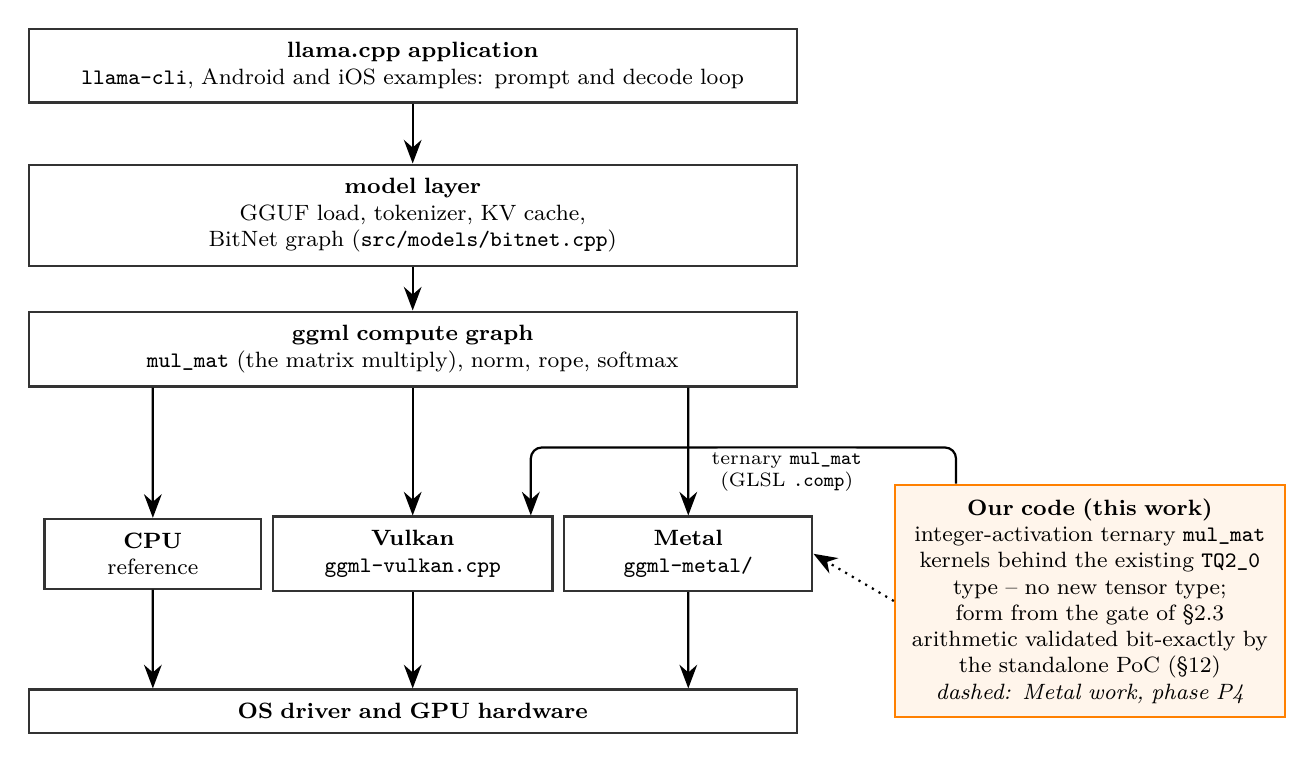
\begin{tikzpicture}
% llama.cpp stack: application -> model layer -> ggml graph -> backends -> device
\node[figbox, text width=9.4cm] (app) at (5.0,9.2) {\textbf{llama.cpp application}\\ \texttt{llama-cli}, Android and iOS examples: prompt and decode loop};
\node[figbox, text width=9.4cm] (model) at (5.0,7.3) {\textbf{model layer}\\ GGUF load, tokenizer, KV cache, \mbox{BitNet} graph (\texttt{src/models/bitnet.cpp})};
\node[figbox, text width=9.4cm] (graph) at (5.0,5.6) {\textbf{ggml compute graph}\\ \texttt{mul\_mat} (the matrix multiply), norm, rope, softmax};
\node[figbox, text width=2.4cm] (cpu) at (1.7,3.0) {\textbf{CPU}\\ reference};
\node[figbox, text width=3.2cm] (vk) at (5.0,3.0) {\textbf{Vulkan}\\ \texttt{ggml-vulkan.cpp}};
\node[figbox, text width=2.8cm] (mtl) at (8.5,3.0) {\textbf{Metal}\\ \texttt{ggml-metal/}};
\node[figbox, text width=9.4cm] (dev) at (5.0,1.0) {\textbf{OS driver and GPU hardware}};
\node[figbox, text width=4.6cm, draw=orange, fill=orange!8] (ours) at (13.6,2.4) {\textbf{Our code (this work)}\\ integer-activation ternary \texttt{mul\_mat}\\ kernels behind the existing \texttt{TQ2\_0}\\ type -- no new tensor type;\\ form from the gate of \S{}2.3\\ arithmetic validated bit-exactly by\\ the standalone PoC (\S{}12)\\ \textit{dashed: Metal work, phase P4}};
\draw[figarrow] (app.south) -- (model.north);
\draw[figarrow] (model.south) -- (graph.north);
\draw[figarrow] ([xshift=-3.3cm]graph.south) -- (cpu.north);
\draw[figarrow] (graph.south) -- (vk.north);
\draw[figarrow] ([xshift=3.5cm]graph.south) -- (mtl.north);
\draw[figarrow] (cpu.south) -- ([xshift=-3.3cm]dev.north);
\draw[figarrow] (vk.south) -- (dev.north);
\draw[figarrow] (mtl.south) -- ([xshift=3.5cm]dev.north);
\draw[figarrow, rounded corners=4pt] ([xshift=-1.7cm]ours.north) |- (6.5,4.35) -- (6.5,0 |- vk.north)
  node[below, align=center, font=\scriptsize, fill=white, inner sep=1.5pt] at (9.75,4.35) {ternary \texttt{mul\_mat}\\ (GLSL \texttt{.comp})};
\draw[figdot] (ours.west) -- (mtl.east);
\end{tikzpicture}
\caption{llama.cpp from application to device, and where this work
enters: integer ternary \texttt{mul\_mat} kernels in the ggml Vulkan and
Metal backends, behind the existing \texttt{TQ2\_0} tensor type}
\end{figure}

\textbf{Where the work lives.} Figure~1 places the kernel work: the
application drives prompt and decode, the model layer builds the BitNet
graph, ggml routes each \texttt{mul\_mat} node to a backend, and the
ternary kernels enter the Vulkan and Metal backends through the existing
\texttt{TQ2\_0} tensor type -- no new tensor type. They enter in the
forms llama.cpp already builds, GLSL and Metal Shading Language
(\S{}2.4). The arithmetic is validated first: the standalone PoC
(\S{}12) computes it bit-exactly against a CPU oracle, and that oracle
guards the adaptation. The converter and model-graph fixes of \S{}2.2
are small edits in the conversion scripts and in the model layer.

\subsection{2.1 Starting point}\label{starting-point}

llama.cpp already contains most of the path: the ternary tensor types
\texttt{TQ1\_0} and \texttt{TQ2\_0} with CPU kernels (PR \#8151), a
BitNet model graph (PR \#7931), Vulkan kernels for both types that
multiply decoded weights with \textbf{floating-point} activations
(\texttt{mul\_mat\_vec\_tq\{1,2\}\_0.comp}, \texttt{matmul\_quant\_*}),
and Metal kernels for \texttt{TQ2\_0}. No new tensor type is proposed.
QVAC Fabric, the task issuer's llama.cpp fork [16], ships BitNet
inference and LoRA fine-tuning on Vulkan and Metal and is the closest
prior art; it shares the model graph discussed below. Outside llama.cpp,
Collabora's ExecuTorch work [17] uses the same 2-bit design point on
Vulkan.

\subsection{2.2 Files and modules to modify or
extend}\label{files-and-modules-to-modify-or-extend}

{\def\LTcaptype{none} % do not increment counter
\begin{longtable}[]{@{}
  >{\raggedright\arraybackslash}p{(\linewidth- 6\tabcolsep) * \real{0.1311}}
  >{\raggedright\arraybackslash}p{(\linewidth- 6\tabcolsep) * \real{0.3443}}
  >{\raggedright\arraybackslash}p{(\linewidth- 6\tabcolsep) * \real{0.2131}}
  >{\raggedright\arraybackslash}p{(\linewidth- 6\tabcolsep) * \real{0.3115}}@{}}
\toprule\noalign{}
\begin{minipage}[b]{\linewidth}\raggedright%
Area
\end{minipage} & \begin{minipage}[b]{\linewidth}\raggedright%
File or module
\end{minipage} & \begin{minipage}[b]{\linewidth}\raggedright%
What exists
\end{minipage} & \begin{minipage}[b]{\linewidth}\raggedright%
Required change
\end{minipage} \\
\midrule\noalign{}
\endhead%
\bottomrule\noalign{}
\endlastfoot%
Conversion & \texttt{gguf-py/gguf/\allowbreak{}tensor\_mapping.py} & sub-norm names
of the older 1bitLLM models & \textbf{add the names of this model}
(\texttt{attn\_sub\_norm}, \texttt{ffn\_sub\_norm}); without them the
conversion fails \\
Conversion & \texttt{conversion/bitnet.py}, \texttt{set\_vocab} &
SentencePiece vocabulary only & \textbf{accept the BPE vocabulary} the
model ships \\
Model graph & \texttt{src/models/bitnet.cpp} & feed-forward block built
with SiLU;\@ model size known for 26 layers only & \textbf{activation from
the model configuration}: this model uses squared ReLU [9, 15].
Measured effect below \\
Vulkan, int8 activations, decode & \texttt{mul\_mat\_vecq.comp},
\texttt{mul\_mat\_vecq\_funcs.glsl}, \texttt{quantize\_q8\_1.comp} (in
\texttt{vulkan-shaders/}); allow-list and pipeline table in
\texttt{ggml-vulkan.cpp}; \texttt{vulkan-shaders-gen.cpp} & integer path
for other quantized types, none for \texttt{TQ} & add a \texttt{TQ2\_0}
kernel with integer activations; variant decided by the gate of \S{}2.3 \\
Vulkan, int8 activations, prompt & \texttt{mul\_mmq.comp},
\texttt{mul\_mmq\_funcs.glsl} (in \texttt{vulkan-shaders/}) & as above &
as above \\
Vulkan, submission & \texttt{ggml-vulkan.cpp}:
\texttt{max\_nodes\_per\_submit} & node-count batching & add a GPU-time
budget per submission (Adreno limit, \S{}1.6) and a dispatch-limit check
per shape \\
Metal (Apple) & in \texttt{ggml/src/ggml-metal/}:
\texttt{ggml-metal-impl.h}, \texttt{ggml-metal-device.cpp},
\texttt{ggml-metal-device.m}, \texttt{kernels/mul\_mv.metal},
\texttt{kernels/mul\_mm.metal}, \texttt{kernels/dequantize.h} &
\texttt{TQ2\_0} kernels; \texttt{TQ1\_0} excluded & \texttt{TQ1\_0}
support, tuning on A-series \\
Quantization tool & \texttt{tools/quantize}, option
\texttt{-{}-token-embedding-type} & exists & documented recipe for the
quantized head (\S{}7); no code change \\
Tests & \texttt{tests/test-backend-ops.cpp} & both \texttt{TQ} types
listed & cases for the new integer kernels; the PoC oracle as the
exactness check \\
Packaging & \texttt{examples/llama.android},
\texttt{examples/llama.swiftui}, \texttt{build-xcframework.sh} & exist &
per-device backend defaults (\S{}6) \\
\end{longtable}
}

\textbf{The three correctness gaps are measured.} The converter fixes
were needed to produce the GGUF at all. The graph defect does not stop
the model from running: it runs at full speed with the wrong activation
function. On the same 16 chunks of WikiText-2 [21]:

{\def\LTcaptype{none} % do not increment counter
\begin{longtable}[]{@{}
  >{\raggedright\arraybackslash}p{(\linewidth- 2\tabcolsep) * \real{0.6471}}
  >{\raggedright\arraybackslash}p{(\linewidth- 2\tabcolsep) * \real{0.3529}}@{}}
\toprule\noalign{}
\begin{minipage}[b]{\linewidth}\raggedright%
Implementation
\end{minipage} & \begin{minipage}[b]{\linewidth}\raggedright%
Perplexity
\end{minipage} \\
\midrule\noalign{}
\endhead%
\bottomrule\noalign{}
\endlastfoot%
Hugging Face \texttt{transformers}, reference implementation [15] &
16.82 $\pm$ 0.78 \\
llama.cpp, upstream graph (SiLU) & 99.31 $\pm$ 5.56 \\
llama.cpp, squared ReLU (one-line change) & 16.80 $\pm$ 0.78 \\
\end{longtable}
}

The patched llama.cpp matches the reference within 0.2\% (same tokens;
the running value after every chunk agrees within 1.2\%). A comparison
of GPU against CPU inside one stack cannot detect this defect, because
both sides share the graph.

\subsection{2.3 Activation quantization: the one open design
decision}\label{activation-quantization-the-one-open-design-decision}

The model is trained with one int8 scale per token (\S{}1.2); llama.cpp
offers other granularities, and a GPU integer kernel has to pick one:

{\def\LTcaptype{none} % do not increment counter
\begin{longtable}[]{@{}
  >{\raggedright\arraybackslash}p{(\linewidth- 6\tabcolsep) * \real{0.1321}}
  >{\raggedright\arraybackslash}p{(\linewidth- 6\tabcolsep) * \real{0.3019}}
  >{\raggedright\arraybackslash}p{(\linewidth- 6\tabcolsep) * \real{0.3396}}
  >{\raggedright\arraybackslash}p{(\linewidth- 6\tabcolsep) * \real{0.2264}}@{}}
\toprule\noalign{}
\begin{minipage}[b]{\linewidth}\raggedright%
Option
\end{minipage} & \begin{minipage}[b]{\linewidth}\raggedright%
Activations
\end{minipage} & \begin{minipage}[b]{\linewidth}\raggedright%
Exists in llama.cpp
\end{minipage} & \begin{minipage}[b]{\linewidth}\raggedright%
Integer kernel
\end{minipage} \\
\midrule\noalign{}
\endhead%
\bottomrule\noalign{}
\endlastfoot%
A & floating point & Vulkan and Metal \texttt{TQ} kernels & no \\
B & int8, one scale per 256 values (\texttt{Q8\_K}) & CPU \texttt{TQ}
kernels & yes \\
C & int8, one scale per 32 values (\texttt{Q8\_1}) & Vulkan integer path
of other types & yes \\
D & int8, one scale per token (training) & no; bitnet.cpp implements the
training scheme on CPUs [4, 5] & yes (the PoC kernels) \\
\end{longtable}
}

Option B is validated: it is what the CPU path computes, and it
reproduces the reference perplexity (table above). Options C and D are
decided in phase P1 by perplexity and KL divergence against the
reference on the CPU, where each is cheap to implement; the GPU kernel
is then built for the cheapest option that passes. The PoC kernels
compute the integer sums all three integer options need.

The option also fixes the form of the GPU kernel. Option C adds
\texttt{TQ2\_0} to the integer path llama.cpp already has: the 2-bit
codes are repacked to int8 lanes in the shader and multiplied with
\texttt{OpSDot} per block of 32 values, the smallest change to upstream
code. Option D needs a new kernel with one integer accumulator per
output and one scale per token, the arithmetic the PoC kernels compute,
and a per-token quantization step. Neither form is measured inside
llama.cpp yet: the PoC's packed-dot kernels read uncompressed int8
weights (\S{}1.3), and the measured GPUs do not report \texttt{OpSDot}
as accelerated, so the ship rule of \S{}6.2 decides per device and role.
The PoC kernels remain the measured reference, and the integer oracle
guards the adaptation.

\needlines{8}
\subsection{2.4 Cross-platform path}\label{cross-platform-path}

{\def\LTcaptype{none} % do not increment counter
\begin{longtable}[]{@{}
  >{\raggedright\arraybackslash}p{(\linewidth- 6\tabcolsep) * \real{0.1600}}
  >{\raggedright\arraybackslash}p{(\linewidth- 6\tabcolsep) * \real{0.1600}}
  >{\raggedright\arraybackslash}p{(\linewidth- 6\tabcolsep) * \real{0.4100}}
  >{\raggedright\arraybackslash}p{(\linewidth- 6\tabcolsep) * \real{0.2700}}@{}}
\toprule\noalign{}
\begin{minipage}[b]{\linewidth}\raggedright%
Platform
\end{minipage} & \begin{minipage}[b]{\linewidth}\raggedright%
Backend
\end{minipage} & \begin{minipage}[b]{\linewidth}\raggedright%
Kernel selection
\end{minipage} & \begin{minipage}[b]{\linewidth}\raggedright%
Entry point
\end{minipage} \\
\midrule\noalign{}
\endhead%
\bottomrule\noalign{}
\endlastfoot%
Android, Mali & Vulkan & pipeline tables in \texttt{ggml-vulkan.cpp}, by
tensor type & \texttt{examples/llama.android} \\
Android, Adreno & Vulkan & as above & \texttt{examples/llama.android} \\
iOS, macOS & Metal & kernel table in \texttt{ggml-metal-device.cpp} &
\texttt{examples/llama.swiftui}, xcframework \\
any & CPU & \texttt{type\_traits\_cpu} & fallback and reference \\
\end{longtable}
}

Slang is the authoring language of the PoC only. What enters llama.cpp
is code in the form it already builds: GLSL \texttt{.comp} sources for
Vulkan and Metal Shading Language for Metal. No new build dependency is
introduced.

\subsection{2.5 Upstream process}\label{upstream-process}

llama.cpp's contribution rules shape the work packages [14]: a
feature starts with an issue; each feature or fix is its own pull
request, with CPU support only in the first; a new contributor may have
one open pull request; the full CI is run locally before a pull request
is published; backend changes need \texttt{test-backend-ops} cases;
model changes need perplexity evidence; AI assistance must be disclosed
and pull-request text is written by the author. The fallback, if
upstream declines a change, is a patch series on QVAC Fabric.

\section{3. Profiling methodology}\label{profiling-methodology}

With the design fixed in \S{}1 and the integration points named in
\S{}2, the next question is how to measure any of it. This section
defines the rules, the instruments and the targets behind every number
in this report.

\subsection{3.1 Principles}\label{principles}

\begin{enumerate}
\def\labelenumi{\arabic{enumi}.}
\tightlist%
\item
  \textbf{A kernel is timed only after it has done its work.} Every
  timed dispatch must first fit the device's dispatch limits and
  reproduce the CPU oracle exactly, starting from an output buffer
  filled with a sentinel value. A negative control in every run
  dispatches half of a grid and requires the check to fail.
\item
  \textbf{The whole pass is measured, not only isolated kernels.} The
  system pass runs the real layer list: 30 layers \texttimes{} 7 projections per
  token plus the output head, one token for decode, 64 tokens for prompt
  processing.
\item
  \textbf{Kernel candidates are compared at system level, twice, in
  opposite order,} so that thermal drift appears as a difference between
  rounds instead of a ranking.
\item
  \textbf{Every log carries its provenance:} UTC time, device serial and
  model, git state, the exact command, CPU/GPU frequency and
  temperatures before and after, the complete program output and the
  exit code.
\item
  \textbf{The GPU is compared with a CPU reference on the same device.}
\end{enumerate}

\subsection{3.2 Instruments}\label{instruments}

{\def\LTcaptype{none} % do not increment counter
\begin{longtable}[]{@{}
  >{\raggedright\arraybackslash}p{(\linewidth- 4\tabcolsep) * \real{0.2500}}
  >{\raggedright\arraybackslash}p{(\linewidth- 4\tabcolsep) * \real{0.3750}}
  >{\raggedright\arraybackslash}p{(\linewidth- 4\tabcolsep) * \real{0.3750}}@{}}
\toprule\noalign{}
\begin{minipage}[b]{\linewidth}\raggedright%
Instrument
\end{minipage} & \begin{minipage}[b]{\linewidth}\raggedright%
Measures
\end{minipage} & \begin{minipage}[b]{\linewidth}\raggedright%
Used for
\end{minipage} \\
\midrule\noalign{}
\endhead%
\bottomrule\noalign{}
\endlastfoot%
\texttt{poc\_tests} & integer equality GPU vs CPU oracle & correctness
gate (\S{}6) \\
\texttt{poc\_bench} matrix & ms per dispatch, 11 kernels \texttimes{} 8 shapes &
kernel candidates \\
\texttt{poc\_bench\ -{}-system} & ms per token, decode and prompt, one
submission per call or per token & throughput upper bound, champion
A/B \\
\texttt{bw\_probe} (GPU kernel) & sustained read bandwidth of the GPU &
memory roof \\
\texttt{alu\_countbits\_probe} (GPU kernel) & rate of the bit-plane
arithmetic with no memory traffic & arithmetic roof \\
\texttt{null\_probe} (GPU kernel) & cost of one submission and fence &
batching decision \\
\texttt{poc\_membw} & read bandwidth of 1..n CPU threads & CPU memory
roof \\
\texttt{llama-bench} & tokens/s of the complete model on the CPU &
reference to beat \\
\texttt{llama-perplexity} & perplexity, KL divergence & accuracy
gates \\
\texttt{malioc} (Arm) & static cycle estimates per shader on Mali &
explaining measurements without device time \\
\end{longtable}
}

Measurement scripts run these instruments step by step on a device and
write one log per step; a summary tool turns the logs into the tables
this report quotes.

\subsection{3.3 Roofline model}\label{roofline-model}

The measurements are read against two ceilings [10]. A token must
read every weight byte once and perform a fixed amount of arithmetic, so

\[
\text{tokens/s} \le\min\left(\frac{B}{\text{bytes per token}},\;
\frac{A}{\text{weights per token}}\right),
\]

with \(B\) the measured read bandwidth (GPU:\@ \texttt{bw\_probe}; CPU:\@
\texttt{poc\_membw}, in the spirit of STREAM [11]) and \(A\) the
measured rate of the kernel's arithmetic
(\texttt{alu\_countbits\_probe}). Both are empirical: the highest rate a
probe reached, not a data-sheet value. The model has 2.084 billion
ternary weights; bytes per token depend on the storage format (\S{}7).

\subsection{3.4 Vendor tools}\label{vendor-tools}

{\def\LTcaptype{none} % do not increment counter
\begin{longtable}[]{@{}
  >{\raggedright\arraybackslash}p{(\linewidth- 4\tabcolsep) * \real{0.1481}}
  >{\raggedright\arraybackslash}p{(\linewidth- 4\tabcolsep) * \real{0.3333}}
  >{\raggedright\arraybackslash}p{(\linewidth- 4\tabcolsep) * \real{0.5185}}@{}}
\toprule\noalign{}
\begin{minipage}[b]{\linewidth}\raggedright%
Platform
\end{minipage} & \begin{minipage}[b]{\linewidth}\raggedright%
Tool
\end{minipage} & \begin{minipage}[b]{\linewidth}\raggedright%
Status
\end{minipage} \\
\midrule\noalign{}
\endhead%
\bottomrule\noalign{}
\endlastfoot%
Mali & Mali Offline Compiler (\texttt{malioc}) & used: e.g.~the
arithmetic probe costs 5.62 cycles on Mali-G57 and 2.08 on Mali-G52,
which with one against two shader cores explains most of the measured
6.8x gap \\
Mali & Streamline / gatord & used for raw bus counters on the Mali-G57;
the per-kernel timeline needs a newer driver (DDK 47, the device has
40) \\
Android & Perfetto & traces captured, not analysed; no statement relies
on them \\
Adreno & Snapdragon Profiler, Android GPU Inspector & planned (P5) \\
Apple & Xcode Instruments, Metal System Trace & planned (P4) \\
\end{longtable}
}

The Android devices are production builds: the Khronos validation layer
cannot be loaded on any of them, and on the two Mali devices the GPU
clock is not readable from a shell process. Device correctness therefore
rests on the integer oracle; the validation layer runs on the desktop.

\subsection{3.5 Metrics and targets}\label{metrics-and-targets}

{\def\LTcaptype{none} % do not increment counter
\begin{longtable}[]{@{}
  >{\raggedright\arraybackslash}p{(\linewidth- 4\tabcolsep) * \real{0.3265}}
  >{\raggedright\arraybackslash}p{(\linewidth- 4\tabcolsep) * \real{0.4898}}
  >{\raggedright\arraybackslash}p{(\linewidth- 4\tabcolsep) * \real{0.1837}}@{}}
\toprule\noalign{}
\begin{minipage}[b]{\linewidth}\raggedright%
Metric
\end{minipage} & \begin{minipage}[b]{\linewidth}\raggedright%
Method
\end{minipage} & \begin{minipage}[b]{\linewidth}\raggedright%
Status
\end{minipage} \\
\midrule\noalign{}
\endhead%
\bottomrule\noalign{}
\endlastfoot%
decode tokens/s, prompt tokens/s & \texttt{poc\_bench\ -{}-system} (GPU
kernels), \texttt{llama-bench} (complete model) & measured \\
bandwidth and arithmetic roofs & probes of \S{}3.2 & measured \\
perplexity, KL divergence & \texttt{llama-perplexity}, reference
implementation & measured for the CPU path and the head formats \\
memory headroom & \texttt{/proc/meminfo} before and after each run &
measured \\
time to first token & \texttt{llama-bench}/\texttt{llama-cli} timings
with the GPU backend & planned (P0) \\
energy per token & battery counters, external power monitor & planned
(P5) \\
sustained rate & 30-minute decode loop with thermal log & planned
(P5) \\
\end{longtable}
}

\textbf{Concrete optimization targets} are derived per device from the
measured bounds and the CPU reference, not chosen freely. Rates in
tokens/s; CPU figures with the Q6\_K output head, the format that passes
the accuracy criterion of \S{}6.2; PoC figures are the linear layers only.

{\def\LTcaptype{none} % do not increment counter
\begin{longtable}[]{@{}
  >{\raggedright\arraybackslash}p{(\linewidth- 6\tabcolsep) * \real{0.3438}}
  >{\raggedright\arraybackslash}p{(\linewidth- 6\tabcolsep) * \real{0.2188}}
  >{\raggedright\arraybackslash}p{(\linewidth- 6\tabcolsep) * \real{0.2188}}
  >{\raggedright\arraybackslash}p{(\linewidth- 6\tabcolsep) * \real{0.2188}}@{}}
\toprule\noalign{}
\begin{minipage}[b]{\linewidth}\raggedright%
Target
\end{minipage} & \begin{minipage}[b]{\linewidth}\raggedright%
Mali-G57 tablet
\end{minipage} & \begin{minipage}[b]{\linewidth}\raggedright%
Mali-G52 tablet
\end{minipage} & \begin{minipage}[b]{\linewidth}\raggedright%
Adreno 740 headset
\end{minipage} \\
\midrule\noalign{}
\endhead%
\bottomrule\noalign{}
\endlastfoot%
Decode on the shipping backend: $\geq$ 75\% of the bandwidth bound (read
bandwidth / 0.807 GB per token) & $\geq$ 3.1; CPU measures 3.58 & $\geq$ 8.7; CPU
measures 5.56 & $\geq$ 27.2; CPU measures 28.8 \\
GPU decode replaces CPU decode: $\geq$ 1.2x CPU, limited by GPU read
bandwidth / bytes per token and by the arithmetic roof & 4.3 needed;
bounds 3.7 (memory) and 1.97 (arithmetic): not reachable & 6.7 needed,
bound 8.0; PoC 4.50 & 34.6 needed, bound 34.1: no margin \\
GPU prompt processing replaces the CPU:\@ $\geq$ 1.2x CPU, limited by the
arithmetic roof & 9.6 needed, roof 1.97: not reachable with this
arithmetic & 12.6 needed, roof 13.4; PoC 5.73 & 64.2 needed, roof 69.8;
PoC 61.5 \\
\end{longtable}
}

The table fixes where optimization effort goes: the CPU decode path on
the Mali-G52 class (48\% of its bound); GPU prompt processing on the
Adreno 740 class, where the PoC kernels reach 88\% of the roof and 92\%
is needed; and the kernel overhead of \S{}5.2 on the Mali-G52 class. The
same derivation is repeated for every device that enters the matrix
(P0).

\section{4. Frameworks, libraries and
SDKs}\label{frameworks-libraries-and-sdks}

{\def\LTcaptype{none} % do not increment counter
\begin{longtable}[]{@{}
  >{\raggedright\arraybackslash}p{(\linewidth- 6\tabcolsep) * \real{0.1724}}
  >{\raggedright\arraybackslash}p{(\linewidth- 6\tabcolsep) * \real{0.2759}}
  >{\raggedright\arraybackslash}p{(\linewidth- 6\tabcolsep) * \real{0.2759}}
  >{\raggedright\arraybackslash}p{(\linewidth- 6\tabcolsep) * \real{0.2759}}@{}}
\toprule\noalign{}
\begin{minipage}[b]{\linewidth}\raggedright%
Purpose
\end{minipage} & \begin{minipage}[b]{\linewidth}\raggedright%
Android: Mali and Adreno
\end{minipage} & \begin{minipage}[b]{\linewidth}\raggedright%
Apple
\end{minipage} & \begin{minipage}[b]{\linewidth}\raggedright%
Used in the PoC
\end{minipage} \\
\midrule\noalign{}
\endhead%
\bottomrule\noalign{}
\endlastfoot%
GPU API & Vulkan 1.1-1.3 (device drivers) & Metal & Vulkan SDK 1.4.363.1
(headers, loader, validation layer) \\
Kernel language & GLSL compiled by llama.cpp's
\texttt{vulkan-shaders-gen} + glslc & Metal Shading Language & Slang
(\texttt{slangc}) $\rightarrow$ SPIR-V, \texttt{spirv-opt}; Slang $\rightarrow$ MSL as a compile
check \\
Inference framework & llama.cpp / ggml (Vulkan, CPU backends) &
llama.cpp / ggml (Metal backend) & llama.cpp for the CPU reference \\
Model conversion & \texttt{convert\_hf\_to\_gguf.py}, \texttt{gguf-py},
\texttt{llama-quantize} & same & same, plus Hugging Face
\texttt{transformers} as reference implementation \\
Build & Android NDK r27 (clang 18), CMake, Ninja & Xcode, CMake & NDK
r27; MSVC 19.51 on the Windows host; CMake 4.4, Ninja 1.13 \\
Deployment & \texttt{adb}, \texttt{examples/llama.android} &
\texttt{examples/llama.swiftui}, xcframework & \texttt{adb} \\
Evaluation & \texttt{llama-bench}, \texttt{llama-perplexity},
\texttt{test-backend-ops} & same & same (CPU), \texttt{poc\_tests},
\texttt{poc\_bench}, \texttt{poc\_membw} \\
Profiling and tuning & Arm Performance Studio (malioc, Streamline),
Perfetto, Android GPU Inspector, Snapdragon Profiler & Xcode
Instruments, Metal System Trace & malioc, Streamline, probes of \S{}3 \\
Code quality & -- & -- & clang-format, clang-tidy, cppcheck, ruff, mypy,
pytest, PSScriptAnalyzer, markdownlint \\
\end{longtable}
}

The PoC has no runtime dependency beyond the Vulkan loader.

\section{5. Kernel-level optimization
strategies}\label{kernel-level-optimization-strategies}

The measurements of \S{}3 produced the numbers. This section turns them
into the strategies that were actually employed, in the order of their
measured leverage, names the candidates that were not adopted and lists
the next steps for the gaps that remain.

\subsection{5.1 What was built and
measured}\label{what-was-built-and-measured}

Eleven kernels in six families (\S{}1.5) were measured over eight shapes of
the model; every row was verified against the oracle before it was
timed. Whole-pass champions, selected by system-level A/B over all
candidates that are legal for every shape of the role, including the
output head:

{\def\LTcaptype{none} % do not increment counter
\begin{longtable}[]{@{}
  >{\raggedright\arraybackslash}p{(\linewidth- 8\tabcolsep) * \real{0.1471}}
  >{\raggedright\arraybackslash}p{(\linewidth- 8\tabcolsep) * \real{0.2647}}
  >{\raggedright\arraybackslash}p{(\linewidth- 8\tabcolsep) * \real{0.1765}}
  >{\raggedright\arraybackslash}p{(\linewidth- 8\tabcolsep) * \real{0.2647}}
  >{\raggedright\arraybackslash}p{(\linewidth- 8\tabcolsep) * \real{0.1471}}@{}}
\toprule\noalign{}
\begin{minipage}[b]{\linewidth}\raggedright%
Device
\end{minipage} & \begin{minipage}[b]{\linewidth}\raggedright%
Decode kernel
\end{minipage} & \begin{minipage}[b]{\linewidth}\raggedright%
ms per token (next candidate)
\end{minipage} & \begin{minipage}[b]{\linewidth}\raggedright%
Prompt kernel
\end{minipage} & \begin{minipage}[b]{\linewidth}\raggedright%
ms per 64 tokens
\end{minipage} \\
\midrule\noalign{}
\endhead%
\bottomrule\noalign{}
\endlastfoot%
Mali-G57 & \texttt{gemv\_plane\_rowcoop} & 573 (684) &
\texttt{gemm\_bitplane\_naive} & 32,353 \\
Mali-G52 & \texttt{gemv\_plane\_rowcoop} & 222 (300) &
\texttt{gemm\_plane\_tiled} & 11,178 \\
Adreno 740 & \texttt{gemv\_bitplane\_ksplit} & 43.5 (46.5) &
\texttt{gemm\_bitplane\_naive} & 1,040 \\
\end{longtable}
}

On Adreno the three cooperative decode kernels are rejected for the
output head (128,256 workgroups against a limit of 65,535), and two
tiled prompt kernels lose the device because one submission exceeds
about 2 s (\S{}1.6).

\subsection{5.2 Where the time goes}\label{where-the-time-goes}

{\def\LTcaptype{none} % do not increment counter
\begin{longtable}[]{@{}llll@{}}
\toprule\noalign{}
Per token, decode & Mali-G57 & Mali-G52 & Adreno 740 \\
\midrule\noalign{}
\endhead%
\bottomrule\noalign{}
\endlastfoot%
measured (ms) & 573 & 222 & 43.5 \\
arithmetic alone, no memory (ms) & 508 & 74.6 & 14.3 \\
weights alone at the GPU read roof (ms) & 176 & 80.7 & 18.9 \\
\textbf{Per 64-token block, prompt} & & & \\
measured (ms) & 32,353 & 11,178 & 1,040 \\
arithmetic alone (ms) & 32,503 & 4,772 & 917 \\
\end{longtable}
}

On the single-core Mali-G57 both roles sit on the arithmetic roof of the
bit-plane method: no memory layout can make these kernels faster there,
only fewer operations per weight. On Adreno 740 prompt processing is
within 13\% of that roof, while decode is 2.3x above the higher of its
two roofs. On Mali-G52 both roles are 2.3-2.8x above the roofs ---
kernel overhead still to be removed.

\subsection{5.3 Strategies employed, in order of measured
leverage}\label{strategies-employed-in-order-of-measured-leverage}

\begin{enumerate}
\def\labelenumi{\arabic{enumi}.}
\tightlist%
\item
  \textbf{Fewer bytes per token.} Decode reads every weight once per
  token. The output head is 55\% of those bytes in f16. Re-encoding it
  at 6.56 or 4.5 bits per weight raised CPU decode by 39-40\% and
  50-54\% on two devices (\S{}7). The same lever applies to a GPU decode
  path, whose bound is also bytes per token.
\item
  \textbf{The right processor per role.} Decode has a ceiling in bytes
  per token: the CPU path reaches 85-91\% of its read bandwidth on two
  devices, and the GPUs measured here read memory more slowly than the
  CPUs (\S{}7); on the Mali-G57 the GPU's arithmetic roof binds even
  earlier (\S{}5.2). Prompt processing is arithmetic-bound; there the
  GPU can win where its arithmetic roof is above the CPU's rate (Adreno
  740: 69.8 against 53.5 tokens/s).
\item
  \textbf{Bit-planes instead of multiply-accumulate.} 16 AND + 16
  popcount per 32 weights; faster than the PoC's packed integer dot
  kernels on all three GPUs in prompt processing and in eight of nine
  decode cases (\S{}1.3).
\item
  \textbf{Wide loads.} Regrouping the planes into 128-bit units (five
  loads per 64 weights) gives the fastest decode kernel on both Mali
  GPUs.
\item
  \textbf{One submission per token, not per call.} Batching the 210
  calls of a token makes decode 1.7x (Mali-G57), 2.8x (Mali-G52) and
  3.2x (Adreno 740) faster than one submission per call. Two effects are
  not separated by the measurement: the per-submission floor (0.2-0.4 ms
  \texttimes{} 210) and the GPU clock dropping between submissions.
\item
  \textbf{Shape-aware dispatch.} Splitting over K with atomics keeps the
  dispatch grid small enough for the 128,256-row head on Adreno;
  submissions are cut below the device's time limit.
\item
  \textbf{Per-device knob profiles as data.} Tile sizes, thread counts
  and the champion per role live in one generated table; a capability
  gate checks every knob and dispatch grid against the device limits
  before any GPU work. Staging K-chunks in workgroup-shared memory is
  such a per-device choice: it is 2.5x faster than the simple prompt
  kernel on Mali-G52 and 1.4x slower on Mali-G57.
\end{enumerate}

Not adopted: lookup-table decoding as in T-MAC [6] (it replaces
arithmetic by loads; not implemented); fused projection shapes (0.8\%
faster decode on Mali-G57 in a run that predates the protocol of \S{}3);
register micro-tiles and a texture-fetch weight path (experimental
kernels, disabled by default). The cooperative-matrix kernel is
disabled: the Slang compiler emits incorrect SPIR-V for int8 cooperative
matrices, which the oracle caught and the validation layer could not.

\subsection{5.4 Next steps for the open gaps}\label{next-steps-for-the-open-gaps}

The gaps of \S{}5.2 set the kernel work of P2 and P3. Nothing in this
list is measured yet.

\begin{itemize}
\tightlist%
\item
  \textbf{Mali-G52: tune on the device first.} Both roles run 2.3-2.8x
  above their roofs, so neither the arithmetic nor the weight reads
  explain the time. The device runs with the knob set of the Mali-G57,
  which fits its limits; only the champions were selected on the
  Mali-G52 itself. A sweep of tile sizes and thread counts on the device
  therefore comes before any kernel change, with static cycle estimates
  (\texttt{malioc}) screening the variants before device time.
\item
  \textbf{Adreno 740: close the last four points in prompt processing.}
  The PoC kernels reach 88\% of the arithmetic roof and 92\% is needed
  (\S{}3.5). The parameters of the two champions on this device are
  constants in the source, not knobs of the profile: workgroups of 16
  \texttimes{} 16 threads in prompt processing, 256 threads and slices
  of 8 words (256 weights) over K in decode. They become knobs and are
  swept on the device. Decode runs 2.3x above the higher of its two
  roofs; the two effects mixed in the batching result, the submission
  floor and the clock dropping between submissions, are separated before
  decode is tuned further.
\item
  \textbf{Mali-G57: fewer operations per weight, as an experiment.} The
  arithmetic roof binds while the memory roof leaves room (176 ms of
  weight reads against 508 ms of arithmetic per token). The candidate is
  the method that trades arithmetic for loads, lookup-table decoding
  [6]. The distance to the target is large: prompt processing needs 9.6
  tokens/s and the roof of the present arithmetic is 1.97 (\S{}3.5), so
  the CPU path remains the plan for this device class.
\end{itemize}

A candidate enters the kernel set only after it reproduces the oracle
and wins the system-level comparison of \S{}3.1. The remaining target of
\S{}3.5 is not a GPU gap: CPU decode on the Mali-G52 class reaches 48\%
of its bound; it is CPU work and belongs to P2, whose exit criterion is
75\% of the bound.

\section{6. Success criteria and evaluation
benchmarks}\label{success-criteria-and-evaluation-benchmarks}

Optimization needs a target, and a target needs a gate. This section
defines what counts as correct for the PoC and what counts as success
for the integration, together with the benchmarks and baselines every
measured number is compared against.

\subsection{6.1 Correctness gates (PoC)}\label{correctness-gates-poc}

{\def\LTcaptype{none} % do not increment counter
\begin{longtable}[]{@{}
  >{\raggedright\arraybackslash}p{(\linewidth- 4\tabcolsep) * \real{0.2500}}
  >{\raggedright\arraybackslash}p{(\linewidth- 4\tabcolsep) * \real{0.5000}}
  >{\raggedright\arraybackslash}p{(\linewidth- 4\tabcolsep) * \real{0.2500}}@{}}
\toprule\noalign{}
\begin{minipage}[b]{\linewidth}\raggedright%
Gate
\end{minipage} & \begin{minipage}[b]{\linewidth}\raggedright%
Criterion
\end{minipage} & \begin{minipage}[b]{\linewidth}\raggedright%
Status
\end{minipage} \\
\midrule\noalign{}
\endhead%
\bottomrule\noalign{}
\endlastfoot%
Integer kernels & GPU output equals the CPU oracle, zero tolerance & met
on four GPUs \\
Known answer & hand-computed vector, expected $\pm$160, through every kernel
& met \\
Real weights & one layer of the model (2560 \texttimes{} 6912), ternarized by the
reference rule, with synthetic activations & met on four GPUs \\
BitLinear forward & float in, reference quantizer, kernel, rescale:
floats equal exactly & met on four GPUs \\
The checks can fail & negative controls reject under-dispatched kernels
& met in every run \\
API usage & Vulkan validation layer, 0 messages & met on the desktop;
not available on the devices \\
Code & zero compiler warnings, static analysis and lint clean
(\texttt{scripts/verify.ps1}) & met \\
\end{longtable}
}

\subsection{6.2 Criteria for the
integration}\label{criteria-for-the-integration}

{\def\LTcaptype{none} % do not increment counter
\begin{longtable}[]{@{}
  >{\raggedright\arraybackslash}p{(\linewidth- 4\tabcolsep) * \real{0.2667}}
  >{\raggedright\arraybackslash}p{(\linewidth- 4\tabcolsep) * \real{0.3667}}
  >{\raggedright\arraybackslash}p{(\linewidth- 4\tabcolsep) * \real{0.3667}}@{}}
\toprule\noalign{}
\begin{minipage}[b]{\linewidth}\raggedright%
Criterion
\end{minipage} & \begin{minipage}[b]{\linewidth}\raggedright%
Target
\end{minipage} & \begin{minipage}[b]{\linewidth}\raggedright%
Basis
\end{minipage} \\
\midrule\noalign{}
\endhead%
\bottomrule\noalign{}
\endlastfoot%
Accuracy of the adaptation & perplexity within 1\% of the reference
implementation on WikiText-2 & measured today: 0.2\% for the CPU path
after the graph fix \\
Integer GPU kernels & bit-exact against the CPU kernel of the same
activation option & PoC oracle \\
Quantized head & mean KL divergence against the f16 head $\leq$ 0.005, same
top token $\geq$ 95\% & Q6\_K measures 0.0017 and 97.1\%; Q4\_K 0.0142 and
91.4\% and does not pass \\
Decode rate, shipping backend & $\geq$ 75\% of the bandwidth bound (read
bandwidth at the same thread count / bytes per token) & the CPU path
measures 79-91\% on two devices, 48-51\% on the Mali-G52 tablet \\
GPU backend ships for a role & $\geq$ 1.2x the tuned CPU path of the same
device in tokens/s, or within 10\% of it at $\geq$ 20\% lower energy per
token & measured CPU reference; energy in P5 \\
Prompt processing on the GPU & Adreno 740 class: $\geq$ 64 tokens/s (1.2x
CPU); per device: \S{}3.5 & PoC upper bound 61.5, arithmetic roof 69.8 \\
Memory & model plus KV cache below the memory available at start; no
page thrashing & Mali-G52 tablet: only the quantized-head files run \\
Sustained rate & $\geq$ 90\% of the initial rate after 30 minutes & P5 \\
\end{longtable}
}

\subsection{6.3 Benchmarks and
baselines}\label{benchmarks-and-baselines}

\begin{itemize}
\tightlist%
\item
  \textbf{Kernel level:} \texttt{poc\_bench}, 11 kernels \texttimes{} 8 shapes of
  the model.
\item
  \textbf{Pass level:} \texttt{poc\_bench\ -{}-system}, decode and
  64-token prompt block.
\item
  \textbf{Model level:} \texttt{llama-bench} (256 prompt tokens, 64
  generated, the threads of the table), \texttt{llama-perplexity} on
  WikiText-2, \texttt{test-backend-ops}.
\item
  \textbf{Baselines:} upstream llama.cpp on the CPU, measured below;
  upstream llama.cpp and QVAC Fabric on the GPU of the same devices,
  measured in P0. Published for the same model [16]: 9.0 tokens/s
  (Pixel 9, Mali GPU) and 5.2 (Galaxy S25, Adreno GPU), with CPU figures
  of 5.2 and 1.8 whose thread count and build flags are not stated.
\end{itemize}

Measured status (tokens/s; GPU = PoC kernels, linear layers only, an
upper bound; CPU = llama.cpp at commit \texttt{93cf736a8d1d} with the
converter fixes, built with \texttt{-march=armv8.2-a+dotprod+fp16},
complete model, best thread count per cell):

{\def\LTcaptype{none} % do not increment counter
\begin{longtable}[]{@{}
  >{\raggedright\arraybackslash}p{(\linewidth- 10\tabcolsep) * \real{0.2807}}
  >{\raggedright\arraybackslash}p{(\linewidth- 10\tabcolsep) * \real{0.1228}}
  >{\raggedright\arraybackslash}p{(\linewidth- 10\tabcolsep) * \real{0.1579}}
  >{\raggedright\arraybackslash}p{(\linewidth- 10\tabcolsep) * \real{0.1579}}
  >{\raggedright\arraybackslash}p{(\linewidth- 10\tabcolsep) * \real{0.1228}}
  >{\raggedright\arraybackslash}p{(\linewidth- 10\tabcolsep) * \real{0.1579}}@{}}
\toprule\noalign{}
\begin{minipage}[b]{\linewidth}\raggedright%
Device
\end{minipage} & \begin{minipage}[b]{\linewidth}\raggedright%
GPU decode
\end{minipage} & \begin{minipage}[b]{\linewidth}\raggedright%
CPU decode, f16 head
\end{minipage} & \begin{minipage}[b]{\linewidth}\raggedright%
CPU decode, Q6\_K head
\end{minipage} & \begin{minipage}[b]{\linewidth}\raggedright%
GPU prompt
\end{minipage} & \begin{minipage}[b]{\linewidth}\raggedright%
CPU prompt
\end{minipage} \\
\midrule\noalign{}
\endhead%
\bottomrule\noalign{}
\endlastfoot%
Mali-G57 MC1, 8\texttimes{} Cortex-A55 & 1.74 & 2.56 & 3.58 & 1.98 & 7.96 \\
Mali-G52 MP2, 2\texttimes{} A75 + 6\texttimes{} A55 & 4.50 & no result & 5.56 & 5.73 & 10.5
(Q6\_K head) \\
Adreno 740, 6\texttimes{} Cortex-A78C & 23.0 & 20.8 & 28.8 & 61.5 & 53.5 \\
\end{longtable}
}

Three details of the CPU reference matter. The build flags: the Arm
dot-product instructions raised prompt processing by 16\% (tablet) and
40\% (headset) over the default build of the NDK.\@ The graph fix of \S{}2.2
does not change speed (21.1 against 20.8 tokens/s decode on the
headset). The thread count: on the Mali-G52 tablet decode peaks at four
threads and collapses at eight (1.1 tokens/s).

\textbf{Today the GPU kernels do not pass the ship rule on any measured
device.} The plan therefore fixes and ships the CPU path first and
develops the GPU path for prompt processing against the criteria above.

\section{7. Hardware constraints; low power, memory bandwidth, compute
overhead}\label{hardware-constraints-low-power-memory-bandwidth-compute-overhead}

The limits below were measured on the test devices before any kernel
was tuned. They explain why the strategies of \S{}5 take the shape they
do, and they bound the low-power, bandwidth and compute budget of the
deployment.

\subsection{7.1 Constraints, measured}\label{constraints-measured}

No phone was available: the constraints are measured on smartphone-class
systems on chip in two tablets and a headset (\S{}12).

{\def\LTcaptype{none} % do not increment counter
\begin{longtable}[]{@{}
  >{\raggedright\arraybackslash}p{(\linewidth- 6\tabcolsep) * \real{0.3077}}
  >{\raggedright\arraybackslash}p{(\linewidth- 6\tabcolsep) * \real{0.2308}}
  >{\raggedright\arraybackslash}p{(\linewidth- 6\tabcolsep) * \real{0.2308}}
  >{\raggedright\arraybackslash}p{(\linewidth- 6\tabcolsep) * \real{0.2308}}@{}}
\toprule\noalign{}
\begin{minipage}[b]{\linewidth}\raggedright%
Constraint
\end{minipage} & \begin{minipage}[b]{\linewidth}\raggedright%
Mali-G57 tablet
\end{minipage} & \begin{minipage}[b]{\linewidth}\raggedright%
Mali-G52 tablet
\end{minipage} & \begin{minipage}[b]{\linewidth}\raggedright%
Adreno 740 headset
\end{minipage} \\
\midrule\noalign{}
\endhead%
\bottomrule\noalign{}
\endlastfoot%
Memory (\texttt{MemTotal}) & 2.72 GiB & 2.42 GiB & 7.58 GiB \\
CPU read bandwidth, best / all cores (GB/s) & 3.91 / 3.37 & 9.35 / 9.28
& 31.9 / 29.3 \\
GPU read bandwidth (GB/s) & 2.96 & 6.46 & 27.5 \\
GPU arithmetic roof (tokens/s) & 1.97 & 13.4 & 69.8 \\
Submission floor (ms) & 0.40 & 0.37 & 0.22 \\
Dispatch groups per axis & 2\textthreesuperior{}\texttwosuperior{}\textminus{}1 & 2\textthreesuperior{}\texttwosuperior{}\textminus{}1 & 65,535 \\
Storage buffer & 256 MiB & 256 MiB & 128 MiB \\
\end{longtable}
}

\textbf{Memory capacity.} Model sizes (from the tensor shapes of the
checkpoint, confirmed by the tensor sizes of the converted file):

{\def\LTcaptype{none} % do not increment counter
\begin{longtable}[]{@{}
  >{\raggedright\arraybackslash}p{(\linewidth- 2\tabcolsep) * \real{0.5833}}
  >{\raggedright\arraybackslash}p{(\linewidth- 2\tabcolsep) * \real{0.4167}}@{}}
\toprule\noalign{}
\begin{minipage}[b]{\linewidth}\raggedright%
Component
\end{minipage} & \begin{minipage}[b]{\linewidth}\raggedright%
Size
\end{minipage} \\
\midrule\noalign{}
\endhead%
\bottomrule\noalign{}
\endlastfoot%
whole model in 16 bit & 4.83 GB:\@ does not fit two of the three
devices \\
ternary layers, \texttt{TQ2\_0} & 0.537 GB \\
embedding = output head (tied), f16 / Q6\_K / Q4\_K & 0.657 / 0.269 /
0.185 GB \\
KV cache, f16, 4096 tokens & 0.315 GB (76.8 kB per token) \\
\end{longtable}
}

On the 2.42 GiB tablet the 1.20 GB file with the f16 head made no
progress in 22 minutes (pages evicted and re-read from storage); the
0.73 GB and 0.82 GB files with a quantized head run. The ternary format
is a necessity on this device class, and the head must be quantized as
well.

\textbf{Memory bandwidth.} With \texttt{TQ2\_0} layers and the f16 head
a token reads 1.19 GB.\@ The CPU path decodes at 2.56 tokens/s on the
Mali-G57 tablet and 20.8 on the headset: 3.06 and 24.9 GB/s of weight
reads, 91\% and 85\% of what the same threads read in the bandwidth
probe. The prediction that follows was tested: with fewer bytes per
token the rate must rise in proportion.

{\def\LTcaptype{none} % do not increment counter
\begin{longtable}[]{@{}
  >{\raggedright\arraybackslash}p{(\linewidth- 8\tabcolsep) * \real{0.1818}}
  >{\raggedright\arraybackslash}p{(\linewidth- 8\tabcolsep) * \real{0.1364}}
  >{\raggedright\arraybackslash}p{(\linewidth- 8\tabcolsep) * \real{0.2727}}
  >{\raggedright\arraybackslash}p{(\linewidth- 8\tabcolsep) * \real{0.2727}}
  >{\raggedright\arraybackslash}p{(\linewidth- 8\tabcolsep) * \real{0.1364}}@{}}
\toprule\noalign{}
\begin{minipage}[b]{\linewidth}\raggedright%
Head format
\end{minipage} & \begin{minipage}[b]{\linewidth}\raggedright%
GB per token
\end{minipage} & \begin{minipage}[b]{\linewidth}\raggedright%
Tablet (8 threads)
\end{minipage} & \begin{minipage}[b]{\linewidth}\raggedright%
Headset (6 threads)
\end{minipage} & \begin{minipage}[b]{\linewidth}\raggedright%
Predicted from bytes
\end{minipage} \\
\midrule\noalign{}
\endhead%
\bottomrule\noalign{}
\endlastfoot%
f16 & 1.194 & 2.56 tok/s & 20.8 tok/s & 1.00 \\
Q6\_K & 0.807 & 3.58 (1.40x) & 28.8 (1.39x) & 1.48x \\
Q4\_K & 0.722 & 3.85 (1.50x) & 32.1 (1.54x) & 1.65x \\
\end{longtable}
}

Prompt processing changes by less than 4\% (it evaluates the head once
per batch). On all three devices the GPU's read bandwidth is below the
CPU's, so a GPU decode path with the same bytes per token has a lower
bound than the CPU path.

\textbf{Compute.} The GPU arithmetic roof is the binding limit on the
single-core Mali-G57 (\S{}5.2).

\textbf{Drivers.} Vulkan versions 1.1 to 1.3, different limits per
vendor (\S{}1.6), no validation layer on the devices, one device loss by
submission time. The PoC checks every limit it depends on at start-up
and fails closed.

\textbf{Thermal and power.} No energy measurement exists yet (P5). Arm's
rule of thumb for DRAM traffic is about 80 mW per GB/s [18]; at the
measured decode traffic this is about 0.25 W on the Mali-G57 tablet and
2 W on the headset, which makes bytes per token an energy lever as well.
Repeat runs at the end of each CPU session reproduced the first decode
rates within 1\%. One prompt-processing run on the headset had a large
spread (47.5 $\pm$ 8.7 tokens/s); the value used is its repeat (53.5 $\pm$ 0.1).

\subsection{7.2 Strategies}\label{strategies}

\begin{itemize}
\tightlist%
\item
  \textbf{Low power:} read fewer bytes per token (quantized head;
  \texttt{TQ1\_0} layers as a further 18\% on the layer bytes, to be
  weighed against its decode arithmetic); one submission per token and
  blocking waits instead of polling; finish prompt processing fast and
  return to idle; choose the backend per role by measured energy per
  token (P5).
\item
  \textbf{Memory bandwidth:} 2-bit weights read once per token with no
  intermediate copies; activations and outputs are kilobytes against
  megabytes of weights; quantized head; KV cache sized to the context
  actually used.
\item
  \textbf{Compute overhead:} bit-plane arithmetic; kernels selected per
  device and role; batched submissions below the device's time limit;
  persistent pipelines and descriptor sets; weights repacked once at
  load, never per token.
\end{itemize}

\section{8. Phased schedule with milestones, deliverables and
checkpoints}\label{phased-schedule-with-milestones-deliverables-and-checkpoints}

Fifty working days (ten working weeks) for one to two
engineers, starting on Tuesday, 1 December 2026; the German public
holidays of the period (25 and 26 December 2026, 1 January 2027) are
not working days, which puts the last day on Wednesday, 10 February
2027. The PoC and the
CPU baselines of this report are the starting point. Each phase ends
with a milestone: its deliverables exist and its exit criterion is met
or the decision rule has been applied. All work happens on our own
branch (a fork of llama.cpp), and the plan ends when that branch is
complete and the pull request is submitted. Upstream takes one open pull
request at a time from a new contributor and asks for CPU support first
(\S{}2.5), so the branch is submitted as a sequence that starts with the
correctness fixes. The review is a discussion with the other developers
of the project and is not predictable, so nothing after the first
submission is scheduled. What the integration takes from the PoC host
code (limit checks, submission budget, oracle test cases, \S{}2.2) is
adapted to C++17 and upstream style in the phase that uses it, with
upstream helpers used where they exist (for example the f16 conversion
helpers of \texttt{ggml.h}); a helper that is missing upstream is added
to the patch, and the PoC itself stays C++23 and standalone.

{\def\LTcaptype{none} % do not increment counter
\begin{longtable}[]{@{}
  >{\raggedright\arraybackslash}p{(\linewidth- 6\tabcolsep) * \real{0.1818}}
  >{\raggedright\arraybackslash}p{(\linewidth- 6\tabcolsep) * \real{0.3333}}
  >{\raggedright\arraybackslash}p{(\linewidth- 6\tabcolsep) * \real{0.2424}}
  >{\raggedright\arraybackslash}p{(\linewidth- 6\tabcolsep) * \real{0.2424}}@{}}
\toprule\noalign{}
\begin{minipage}[b]{\linewidth}\raggedright%
Phase, working days, dates
\end{minipage} & \begin{minipage}[b]{\linewidth}\raggedright%
Deliverables
\end{minipage} & \begin{minipage}[b]{\linewidth}\raggedright%
Milestone: exit criterion
\end{minipage} & \begin{minipage}[b]{\linewidth}\raggedright%
Decision rule
\end{minipage} \\
\midrule\noalign{}
\endhead%
\bottomrule\noalign{}
\endlastfoot%
\textbf{P0} Baselines and correctness; 5 days, 1-7 Dec & issue upstream;
converter fixes and graph activation on our own branch; upstream and
QVAC Fabric GPU baselines on the device matrix; perplexity/KL pipeline
on the full WikiText-2 test split & llama.cpp within 1\% of the
reference perplexity; baseline table committed & a device whose GPU
backend fails stays on the CPU path \\
\textbf{P1} Accuracy decisions; 5 days, 8-14 Dec & activation options B,
C, D on the CPU;\@ head formats with and without importance matrix &
decision record with perplexity and KL per option & no integer option
passes: keep floating-point activations (A) \\
\textbf{P2} Decode; 10 days, 15-29 Dec & quantized-head model recipe and
CPU defaults (threads, build flags); GPU decode kernel for the chosen
option; the PoC's oracle test cases adapted to C++17 for
\texttt{test-backend-ops}; backend decision per device & decode $\geq$
75\% of the bandwidth bound on the shipping backend; new kernels
bit-exact and in \texttt{test-backend-ops} & GPU decode below the ship
rule: CPU decode ships, GPU work continues for prompt processing only \\
\textbf{P3} Prompt processing; 10 days, 30 Dec to 13 Jan &
\texttt{TQ2\_0} integer prompt kernel with the PoC arithmetic;
time-budgeted submissions and dispatch-limit checks, adapted to C++17
from the PoC host code & GPU prompt $\geq$ 1.2x CPU
on the Adreno 740 class & below 1.2x: tune or drop per device; no device
blocks the submission \\
\textbf{P4} Apple; 5 days, 14-20 Jan & \texttt{TQ1\_0} in Metal, tuning
and measurements on A-series hardware & bit-exact kernels; baseline
table for one iPhone & no hardware: the phase follows P6, outside this
schedule \\
\textbf{P5} Power and thermal; 5 days, 21-27 Jan & energy per token per
backend and role; 30-minute soak; backend policy per device class &
sustained rate $\geq$ 90\%; policy table & -- \\
\textbf{P6} Pull request; 10 days, 28 Jan to 10 Feb & accuracy sign-off on
the device matrix; Android and iOS examples with the per-device
defaults; the branch cut into the pull-request sequence and its first
pull request submitted (or the QVAC patch set) & all criteria of
\S{}6.2 reported per device; the local CI run and
\texttt{test-backend-ops} pass on the branch & upstream declines: QVAC
patch series \\
\end{longtable}
}

\begin{figure}
\centering
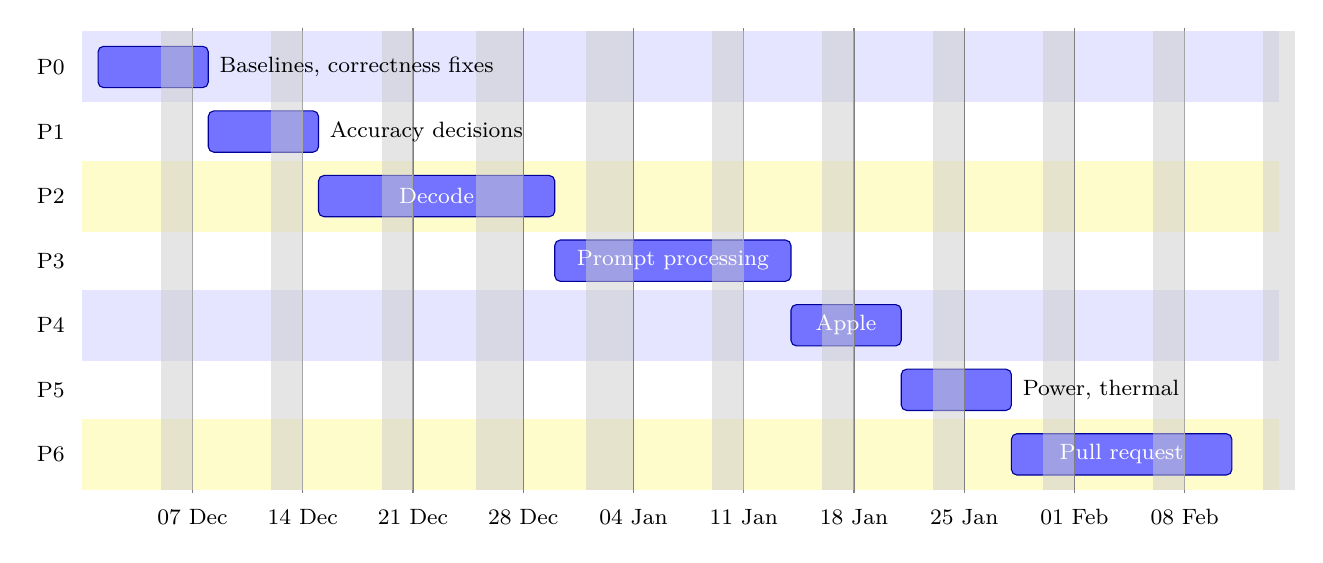
\begin{tikzpicture}[x=0.2cm, y=0.82cm, font=\footnotesize]
% row bands (alternating section tint, as in the original chart)
\fill[blue!10]  (0, 0.55) rectangle (76,-0.55);
\fill[yellow!20] (0,-1.45) rectangle (76,-2.55);
\fill[blue!10]  (0,-3.45) rectangle (76,-4.55);
\fill[yellow!20] (0,-5.45) rectangle (76,-6.55);
% bars: working-day durations of the plan, converted to calendar spans
\draw[ganttbar] (1,0.32)   rectangle (8,-0.32);
\draw[ganttbar] (8,-0.68)  rectangle (15,-1.32);
\draw[ganttbar] (15,-1.68) rectangle (30,-2.32);
\draw[ganttbar] (30,-2.68) rectangle (45,-3.32);
\draw[ganttbar] (45,-3.68) rectangle (52,-4.32);
\draw[ganttbar] (52,-4.68) rectangle (59,-5.32);
\draw[ganttbar] (59,-5.68) rectangle (73,-6.32);
% weekly gridlines (Mondays) and axis labels
\foreach\d/\lab in {7/07 Dec, 14/14 Dec, 21/21 Dec, 28/28 Dec, 35/04 Jan,
  42/11 Jan, 49/18 Jan, 56/25 Jan, 63/01 Feb, 70/08 Feb}{
  \draw[black!50, thin] (\d,0.6) -- (\d,-6.6);
  \node[anchor=north] at (\d,-6.7) {\lab};}
% weekends and public holidays (25 December, 1 January): shaded over the
% bars, so the shaded days extend the phases they fall into
\foreach\d in {5,6,12,13,19,20,25,26,27,32,33,34,40,41,47,48,54,55,61,62,
  68,69,75,76}
  \fill[black!20, opacity=0.5] (\d,0.55) rectangle (\d+1,-6.55);
% row labels
\foreach\i in {0,1,2,3,4,5,6} \node[anchor=east] at (-0.5,-\i) {P\i};
% bar labels: inside when the bar is wide enough, else right of the bar
\node[anchor=west] at (8.1,0) {Baselines, correctness fixes};
\node[anchor=west] at (15.1,-1) {Accuracy decisions};
\node[text=white] at (22.5,-2) {Decode};
\node[text=white] at (37.5,-3) {Prompt processing};
\node[text=white] at (48.5,-4) {Apple};
\node[anchor=west] at (59.1,-5) {Power, thermal};
\node[text=white] at (66,-6) {Pull request};
\end{tikzpicture}
\caption{Schedule from 1 December 2026 to 10 February 2027. Weekends and
the public holidays (25 December, 1 January) are shaded and extend the
phases they fall into.}
\end{figure}

\textbf{Progress tracking checkpoints.} Weekly: the measurement scripts
regenerate the status table of \S{}6.3 for the device matrix from raw logs;
a number without a log does not enter a report. At each milestone: a
review against the exit criterion; the reviews that close P0 to P3 (7,
14 and 29 December, 13 January) are go/no-go decisions by the decision
rule of the phase.

\section{9. Risks and mitigations}\label{risks-and-mitigations}

{\def\LTcaptype{none} % do not increment counter
\begin{longtable}[]{@{}
  >{\raggedright\arraybackslash}p{(\linewidth- 6\tabcolsep) * \real{0.2500}}
  >{\raggedright\arraybackslash}p{(\linewidth- 6\tabcolsep) * \real{0.1562}}
  >{\raggedright\arraybackslash}p{(\linewidth- 6\tabcolsep) * \real{0.3438}}
  >{\raggedright\arraybackslash}p{(\linewidth- 6\tabcolsep) * \real{0.2500}}@{}}
\toprule\noalign{}
\begin{minipage}[b]{\linewidth}\raggedright%
Risk
\end{minipage} & \begin{minipage}[b]{\linewidth}\raggedright%
Likelihood / impact
\end{minipage} & \begin{minipage}[b]{\linewidth}\raggedright%
Mitigation
\end{minipage} & \begin{minipage}[b]{\linewidth}\raggedright%
Contingency
\end{minipage} \\
\midrule\noalign{}
\endhead%
\bottomrule\noalign{}
\endlastfoot%
GPU slower than the CPU for decode & measured on three devices / high &
ship rule per device and role (\S{}6.2); bytes-per-token work benefits both
& CPU decode, GPU for prompt processing only \\
GPU prompt processing does not reach 1.2x & medium / medium & arithmetic
roof measured per device before any adaptation; kernels within 13\% of
the roof on Adreno 740 & CPU path on that device class \\
Wrong results that run at full speed (graph defect class) & occurred /
high & reference-implementation perplexity as the first gate (P0);
integer oracle for kernels & -- \\
Head quantization costs accuracy & medium / medium & KL gate (\S{}6.2);
Q6\_K passes on a 16-chunk sample, to be confirmed on the full split &
f16 head on devices with enough memory \\
Driver limits and defects (dispatch count, buffer size, submission time,
missing validation layer) & certain / medium & capability gate that
fails closed; desktop validation lane; integer oracle on every device &
CPU path \\
Measurement errors & occurred / high & timing only after oracle
verification, negative controls, generated summaries & re-measure and
correct the affected statements \\
No Apple hardware; one device per Android GPU family & certain / medium
& statements about unmeasured devices are marked; P0 and P4 extend the
matrix & Apple phase after the submission \\
Memory pressure on 3 GB devices & measured / high & quantized head,
context limit, memory check before load & smaller context;
\texttt{TQ1\_0} layers \\
Upstream review latency or rejection & medium / medium & issue opened in
P0; small sequential pull requests with evidence, cut from the finished
branch & QVAC Fabric patch series \\
Our branch drifts from upstream master, which moves daily (\S{}10) &
certain / medium & rebase at every milestone, then repeat the reference
perplexity and \texttt{test-backend-ops}; file names and gaps
re-verified & final rebase in P6 before the submission \\
Thermal throttling distorts numbers & medium / medium & device state in
every log, repeat runs, 30-minute soak in P5 & report sustained rates \\
\end{longtable}
}

\section{10. Assumptions and
dependencies}\label{assumptions-and-dependencies}

\textbf{Model.} The team's model is assumed to have the architecture of
\texttt{microsoft/bitnet-b1.58-2B-4T} (verified from the checkpoint): 30
layers, hidden size 2560, feed-forward size 6912, 20 attention heads
with 5 key/value heads, vocabulary 128,256, tied embeddings, context
4096, squared-ReLU activation, 2,412,820,480 parameters of which
2,084,044,800 are ternary. A different activation, vocabulary or
sub-norm naming changes the converter and graph work of \S{}2.2, not the
kernels.

\textbf{Software.} llama.cpp master moves daily; file names and gaps
were verified at the commits named in \S{}2 and must be re-verified when
work starts. QVAC Fabric is assumed to remain a llama.cpp fork that can
take the same patches. The Vulkan drivers of the target devices are
assumed to offer what the kernels need: Vulkan 1.0 with popcount for the
bit-plane kernels; everything else is checked at run time.

\textbf{Hardware.} Three Android devices and one desktop GPU were
measured (\S{}12). Statements about other devices, in particular
current flagship phones and all Apple hardware, are not measurements.
The schedule assumes access to one iPhone and at least one current
flagship Android phone from P0.

\textbf{People and process.} One to two engineers. Upstream takes one
open pull request at a time from a new contributor; how long its review
takes is not predictable and is outside the schedule (\S{}8).

\section{11. Other information and
constraints}\label{other-information-and-constraints}

\begin{itemize}
\tightlist%
\item
  \textbf{Scope of the PoC numbers.} The GPU rates are upper bounds:
  linear layers only, without attention, normalization, sampling and the
  quantization of activations between layers; the 30 layers reuse the
  buffers of one layer, so memory capacity is not exercised; the PoC's
  output head is a 2-bit stand-in. The CPU rates are complete model
  runs.
\item
  \textbf{Sample sizes.} Perplexity and KL figures use 16 chunks (4,080
  scored tokens) of WikiText-2; they decide nothing finally and are
  repeated on the full split in P0/P1.
\item
  \textbf{Not measured:} energy, time to first token on the GPU, Apple
  hardware, the upstream and QVAC GPU backends on these devices.
\item
  \textbf{Prior art.} No technique in this work is new; the references
  name the sources. The contribution is the verified implementation, the
  measurements and the plan.
\item
  \textbf{Reproducibility.} Every measured number in this report comes
  from a log written by the measurement protocol of \S{}3.1. The logs,
  the measurement scripts and the summary tool are not part of the
  delivery. The proof of concept builds and runs from the delivered
  source; \texttt{README.md} is its entry point.
\item
  \textbf{Authorship.} Developed with AI assistance under the author's
  direction and review.\ \copyright{} 2026 Norbert Nopper, MIT license.
\end{itemize}

\section{12. Proof of concept}\label{proof-of-concept}

\textbf{Kernel.} Ternary (and 1-bit) matrix multiplication in Vulkan
compute for one BitLinear layer: int8 activations \texttimes{} packed ternary
weights $\rightarrow$ int32 accumulators, exactly as \S{}1.2-1.3. Eleven kernels in one
Slang source, compiled per GPU profile.

% Set as a fixed block in its reading position, not as a float: as a
% float it was pushed behind the text of this section.
\par\medskip
\noindent\begin{minipage}{\linewidth}
\centering
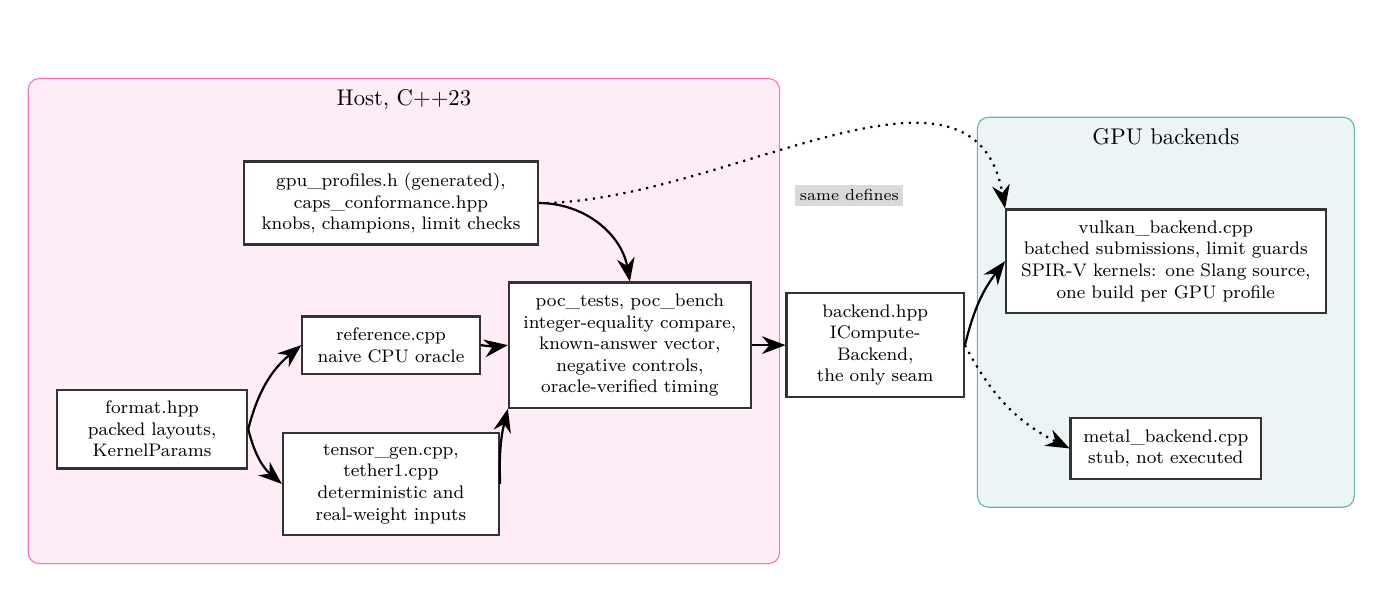
\begin{tikzpicture}[scale=0.82, transform shape]
% content cross-checked against the ground truth: the original mermaid
\node[figbox, text width=2.6cm] (F) at (1.7,1.0) {format.hpp\\ packed layouts,\\ KernelParams};
\node[figbox, text width=4.2cm] (P) at (5.4,4.5) {gpu\_profiles.h (generated),\\ caps\_conformance.hpp\\ knobs, champions, limit checks};
\node[figbox, text width=3.0cm] (I) at (5.4,0.15) {tensor\_gen.cpp, tether1.cpp\\ deterministic and\\ real-weight inputs};
\node[figbox, text width=2.4cm] (R) at (5.4,2.3) {reference.cpp\\ naive CPU oracle};
\node[figbox, text width=3.4cm] (H) at (9.1,2.3) {poc\_tests, poc\_bench\\ integer-equality compare,\\ known-answer vector,\\ negative controls,\\ oracle-verified timing};
\node[figbox, text width=2.4cm] (B) at (12.9,2.3) {backend.hpp\\ IComputeBackend,\\ the only seam};
\node[figbox, text width=4.6cm] (V) at (17.4,3.6) {vulkan\_backend.cpp\\ batched submissions, limit guards\\ SPIR-V kernels: one Slang source,\\ one build per GPU profile};
\node[figbox, text width=2.6cm] (M) at (17.4,0.7) {metal\_backend.cpp\\ stub, not executed};
% subgraph containers (phantom anchor above the widest box, drawn behind)
\node[coordinate] (hosttitle) at (9.9,6.0) {};
\node[coordinate] (gputitle) at (17.4,5.4) {};
\begin{scope}[on background layer]
  \node[figsub, draw=magenta!55, fill=magenta!7, fit=(F)(P)(I)(R)(H)(hosttitle)] (host) {};
  \node[figsub, draw=teal!60, fill=teal!8, fit=(V)(M)(gputitle)] (gpu) {};
\end{scope}
\node[anchor=north, inner sep=2pt] at ([yshift=-3pt]host.north) {Host, C++23};
\node[anchor=north, inner sep=2pt] at ([yshift=-3pt]gpu.north) {GPU backends};
\draw[figarrow] (F.east) to[bend right=18] (I.west);
\draw[figarrow] (F.east) to[bend left=18] (R.west);
\draw[figarrow] (P.east) to[out=0, in=100] (H.north);
\draw[figarrow] (R.east) to[bend right=8] (H.west);
\draw[figarrow] (I.east) to[bend left=8] (H.south west);
\draw[figarrow] (H.east) -- (B.west);
\draw[figarrow] (B.east) to[bend left=12] (V.west);
\draw[figdot] (B.east) to[bend right=18] (M.west);
\draw[figdot] (P.east) to[out=0, in=100] (V.north west);
\node[fill=black!15, inner sep=2pt, font=\scriptsize] at (12.5,4.62) {same defines};
\end{tikzpicture}
\makeatletter\def\@captype{figure}\makeatother
\caption{PoC architecture: format contract, CPU oracle, harness,
generated profile table, one backend seam}
\end{minipage}
\par\medskip

\textbf{Test harness (\texttt{poc\_tests}).} For every shape the harness
generates deterministic inputs, computes the reference with a naive CPU
loop, runs every kernel on the GPU and requires equal int32 outputs
(differential testing [12]).

{\def\LTcaptype{none} % do not increment counter
\begin{longtable}[]{@{}
  >{\raggedright\arraybackslash}p{(\linewidth- 2\tabcolsep) * \real{0.3548}}
  >{\raggedright\arraybackslash}p{(\linewidth- 2\tabcolsep) * \real{0.6452}}@{}}
\toprule\noalign{}
\begin{minipage}[b]{\linewidth}\raggedright%
Sample input / output validation
\end{minipage} & \begin{minipage}[b]{\linewidth}\raggedright%
Content
\end{minipage} \\
\midrule\noalign{}
\endhead%
\bottomrule\noalign{}
\endlastfoot%
Known-answer vector (\texttt{data/golden\_vector.txt}) & \(K = 64\);
activations \(+3, -2, +3, -2, \dots\); weights \(w_{ij} = +1\) if
\(i + j\) even, else \(-1\); expected output \(+160\) for even \(i\),
\(-160\) for odd \(i\) (\(32 \cdot3 + 32 \cdot2\)), checked against
the file, the closed form and every kernel \\
Synthetic shapes & 9 single-token and 11 multi-token shapes: the layer
shapes of the model, odd sizes (\(K\) from 1 to 513, 1 to 65 tokens),
extreme values (+127/\textminus{}128), all zeros, 1-bit weights \{\textminus{}1, +1\} \\
Real weights & layer 12 \texttt{down\_proj} of the model (2560 \texttimes{} 6912),
ternarized with the reference formula (checked element-wise by a Python
test), 8 tokens of seeded synthetic int8 activations; the container is
recreated by
\texttt{tools/export\_weights.py} into \texttt{models/}, selected with
\texttt{poc\_tests\ -{}-tensors\ \textless{}container\textgreater{}} \\
BitLinear forward & float activations $\rightarrow$ reference quantizer $\rightarrow$ kernel $\rightarrow$
rescaling; 20,480 float outputs equal on GPU and CPU paths \\
Negative controls & a deliberately under-dispatched kernel must fail the
comparison \\
\end{longtable}
}

\textbf{Result:} \texttt{ALL\ TESTS\ PASSED} on the four GPUs, 111
kernel \texttimes{} shape checks each plus the known-answer, real-weight and
BitLinear cases.

{\def\LTcaptype{none} % do not increment counter
\begin{longtable}[]{@{}
  >{\raggedright\arraybackslash}p{(\linewidth- 6\tabcolsep) * \real{0.2500}}
  >{\raggedright\arraybackslash}p{(\linewidth- 6\tabcolsep) * \real{0.2188}}
  >{\raggedright\arraybackslash}p{(\linewidth- 6\tabcolsep) * \real{0.3438}}
  >{\raggedright\arraybackslash}p{(\linewidth- 6\tabcolsep) * \real{0.1875}}@{}}
\toprule\noalign{}
\begin{minipage}[b]{\linewidth}\raggedright%
Device
\end{minipage} & \begin{minipage}[b]{\linewidth}\raggedright%
CPU
\end{minipage} & \begin{minipage}[b]{\linewidth}\raggedright%
GPU, driver, Vulkan
\end{minipage} & \begin{minipage}[b]{\linewidth}\raggedright%
Role
\end{minipage} \\
\midrule\noalign{}
\endhead%
\bottomrule\noalign{}
\endlastfoot%
Windows desktop & Intel Core Ultra 7 265F & NVIDIA RTX 5070, 621.24,
1.4.357 & correctness with validation layer \\
MUJENYZ A9 tablet (Allwinner A523) & 8\texttimes{} Cortex-A55 & Mali-G57 MC1, DDK
40, 1.3.225 & budget target \\
Galaxy Tab A8 (Unisoc T618) & 2\texttimes{} Cortex-A75 + 6\texttimes{} Cortex-A55 & Mali-G52
MP2, DDK 34, 1.1.191 & older Mali \\
Meta Quest 3 (Snapdragon XR2 Gen 2) & 6\texttimes{} Cortex-A78C & Adreno 740,
512.837.9, 1.3.295 & Adreno \\
\end{longtable}
}

The shader-core counts (MC1, MP2) are those of the SoC specifications;
the drivers do not report them. Desktop timings are reference values
only: the machine is a shared workstation, and within one run the time
of the same pass spreads by more than a factor of two (output head: 22.3
ms minimum, 51.0 ms at the 90th percentile). Build and run instructions
are in \texttt{README.md}.

% The UML figure is set as a fixed block at the end of the section, not
% as a float: as a float it was pushed to a page of its own, which left
% the end of this section on a nearly empty page. \@captype makes
% \caption work outside a float.
\par\medskip
\noindent\begin{minipage}{\linewidth}
\centering
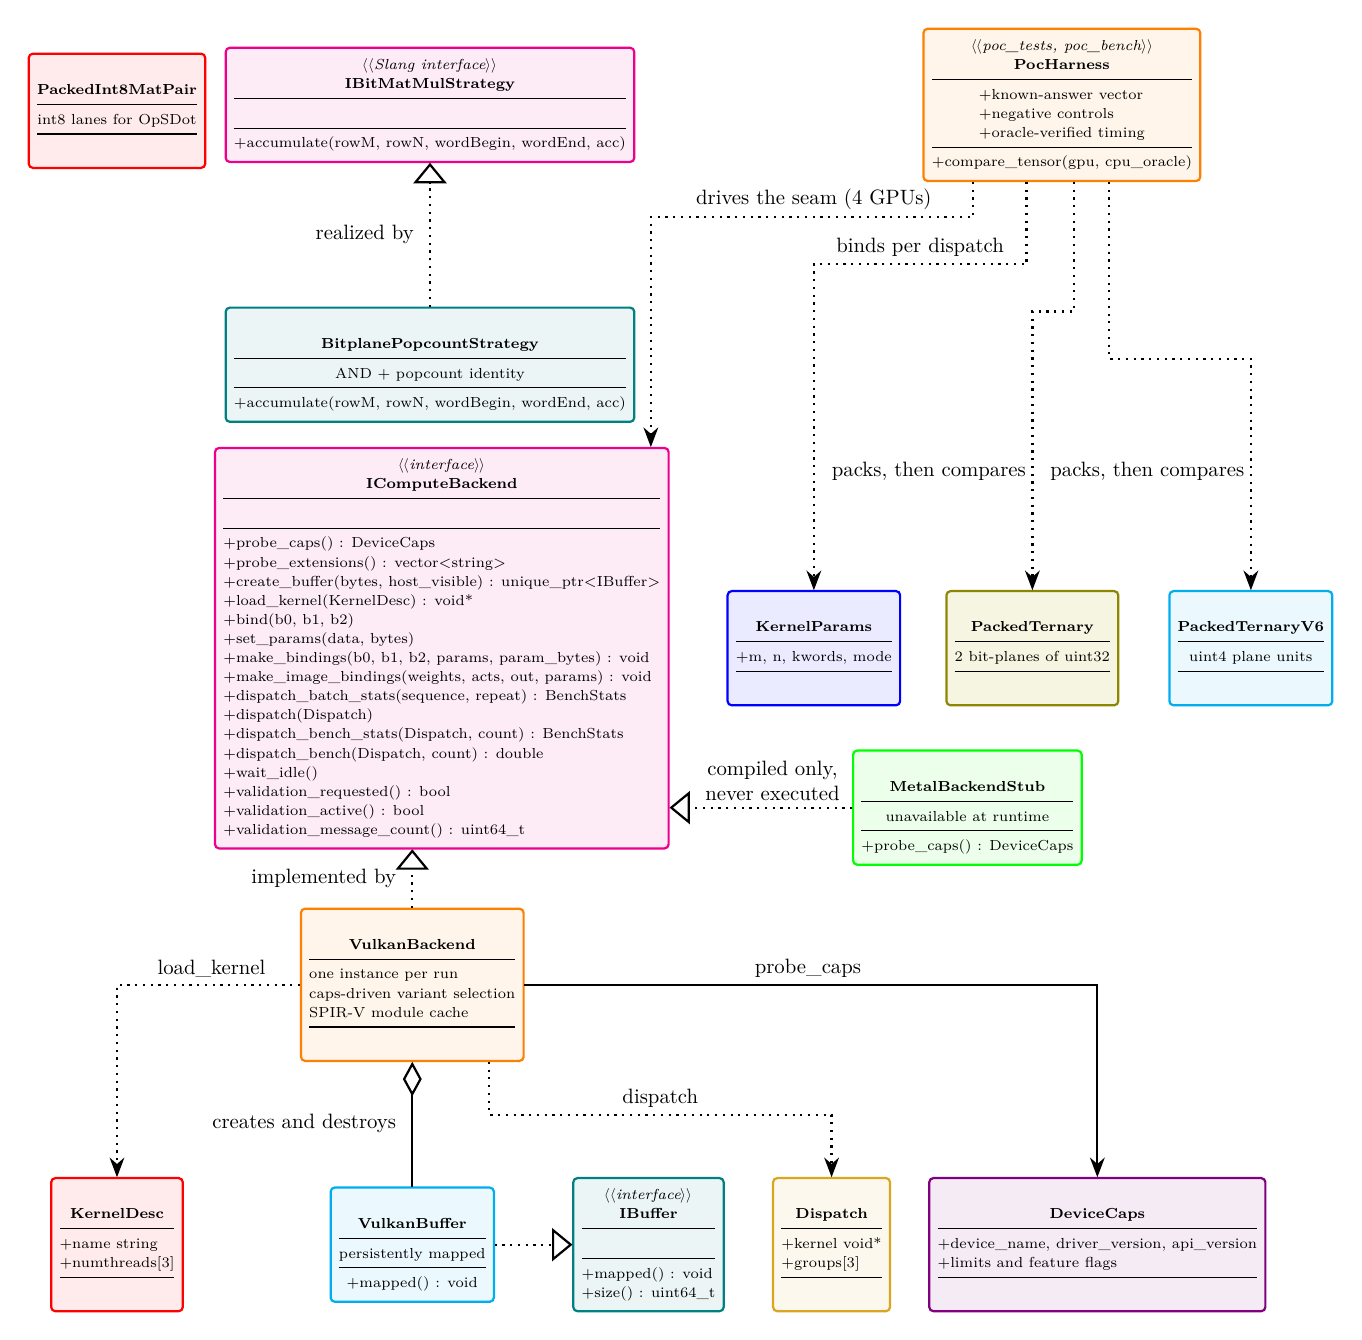
\begin{tikzpicture}[scale=0.75, transform shape]
% content cross-checked against the ground truth: the original mermaid
\umlclass{p8mat}{(1.6,14.1)}{red}{}{PackedInt8MatPair}{int8 lanes for OpSDot}{\phantom{m}}
\umlclass{strategy}{(6.9,14.2)}{magenta}{$\langle\langle$Slang interface$\rangle\rangle$}{IBitMatMulStrategy}{\phantom{m}}{+accumulate(rowM, rowN, wordBegin, wordEnd, acc)}
\umlclass{poc}{(17.6,14.2)}{orange}{$\langle\langle$poc\_tests, poc\_bench$\rangle\rangle$}{PocHarness}{+known-answer vector \\ +negative controls \\ +oracle-verified timing}{+compare\_tensor(gpu, cpu\_oracle)}
\umlclass{bitplane}{(6.9,9.8)}{teal}{}{BitplanePopcountStrategy}{AND + popcount identity}{+accumulate(rowM, rowN, wordBegin, wordEnd, acc)}
\umlclass{icb}{(7.1,5.0)}{magenta}{$\langle\langle$interface$\rangle\rangle$}{IComputeBackend}{\phantom{m}}{+probe\_caps() : DeviceCaps \\ +probe\_extensions() : vector\textless{}string\textgreater{} \\ +create\_buffer(bytes, host\_visible) : unique\_ptr\textless{}IBuffer\textgreater{} \\ +load\_kernel(KernelDesc) : void* \\ +bind(b0, b1, b2) \\ +set\_params(data, bytes) \\ +make\_bindings(b0, b1, b2, params, param\_bytes) : void \\ +make\_image\_bindings(weights, acts, out, params) : void \\ +dispatch\_batch\_stats(sequence, repeat) : BenchStats \\ +dispatch(Dispatch) \\ +dispatch\_bench\_stats(Dispatch, count) : BenchStats \\ +dispatch\_bench(Dispatch, count) : double \\ +wait\_idle() \\ +validation\_requested() : bool \\ +validation\_active() : bool \\ +validation\_message\_count() : uint64\_t}
\umlclass{kparams}{(13.4,5.0)}{blue}{}{KernelParams}{+m, n, kwords, mode}{\phantom{m}}
\umlclass{pt}{(17.1,5.0)}{olive}{}{PackedTernary}{2 bit-planes of uint32}{\phantom{m}}
\umlclass{ptv6}{(20.8,5.0)}{cyan}{}{PackedTernaryV6}{uint4 plane units}{\phantom{m}}
\umlclass{vbackend}{(6.6,-0.7)}{orange}{}{VulkanBackend}{one instance per run \\ caps-driven variant selection \\ SPIR-V module cache}{\phantom{m}}
\umlclass{metal}{(16.0,2.3)}{green}{}{MetalBackendStub}{unavailable at runtime}{+probe\_caps() : DeviceCaps}
\umlclass{ibuf}{(10.6,-5.1)}{teal}{$\langle\langle$interface$\rangle\rangle$}{IBuffer}{\phantom{m}}{+mapped() : void \\ +size() : uint64\_t}
\umlclass{kdesc}{(1.6,-5.1)}{red}{}{KernelDesc}{+name string \\ +numthreads[3]}{\phantom{m}}
\umlclass{vbuf}{(6.6,-5.1)}{cyan}{}{VulkanBuffer}{persistently mapped}{+mapped() : void}
\umlclass{dispatch}{(13.7,-5.1)}{Goldenrod}{}{Dispatch}{+kernel void* \\ +groups[3]}{\phantom{m}}
\umlclass{caps}{(18.2,-5.1)}{violet}{}{DeviceCaps}{+device\_name, driver\_version, api\_version \\ +limits and feature flags}{\phantom{m}}
% relations (labels as in the ground-truth diagram). Every line starts and
% ends on a node anchor, so it meets the box edge whatever the box size is.
\draw[umldep] (16.1,0 |- poc.south) -- (16.1,12.3) -- (10.64,12.3) -- (10.64,0 |- icb.north);
\node[above] at (13.4,12.3) {drives the seam (4 GPUs)};
\draw[umldep] (17.0,0 |- poc.south) -- (17.0,11.5) -- (kparams.north |- 0,11.5) -- (kparams.north);
\node[above] at (15.2,11.5) {binds per dispatch};
\draw[umldep] (17.8,0 |- poc.south) -- (17.8,10.7) -- (pt.north |- 0,10.7) -- (pt.north);
\node[left, fill=white, inner sep=1.5pt] at (17.05,8.0) {packs, then compares};
\draw[umldep] (18.4,0 |- poc.south) -- (18.4,9.9) -- (ptv6.north |- 0,9.9) -- (ptv6.north);
\node[left, fill=white, inner sep=1.5pt] at (20.75,8.0) {packs, then compares};
\draw[umlreal] (bitplane.north) -- (strategy.south);
\node[left] at (6.75,12.0) {realized by};
\draw[umlreal] (vbackend.north) -- (vbackend.north |- icb.south);
\node[left] at (6.45,1.1) {implemented by};
\draw[umlreal] (metal.west) -- (icb.east |- metal.west);
\node[above, align=center] at (12.7,2.3) {compiled only,\\ never executed};
\draw[umlreal] (vbuf.east) -- (ibuf.west |- vbuf.east);
\draw[umlagg] (vbackend.south) -- (vbuf.north);
\node[left] at (6.45,-3.05) {creates and destroys};
\draw[umldep] (vbackend.west) -- (kdesc.north |- vbackend.west) -- (kdesc.north);
\node[above] at (3.2,-0.7) {load\_kernel};
\draw[umldep] (7.9,0 |- vbackend.south) -- (7.9,-2.9) -- (dispatch.north |- 0,-2.9) -- (dispatch.north);
\node[above] at (10.8,-2.9) {dispatch};
\draw[umlsolid] (vbackend.east) -- (caps.north |- vbackend.east) -- (caps.north);
\node[above] at (13.3,-0.7) {probe\_caps};
\end{tikzpicture}
\makeatletter\def\@captype{figure}\makeatother
\caption{UML class diagram of the proof of concept: the IComputeBackend
seam and its two implementations, the packed format contract, the
compile-time strategy interface and the test harness}
\end{minipage}

% The references start on a fresh page.
\clearpage
\section{References}\label{references}

\begin{enumerate}
\def\labelenumi{\arabic{enumi}.}
\tightlist%
\item
  S. Ma et al., ``The Era of 1-bit LLMs: All Large Language Models are
  in 1.58 Bits'', arXiv:2402.17764, 2024.
  \url{https://arxiv.org/abs/2402.17764}
\item
  H. Wang et al., ``BitNet: Scaling 1-bit Transformers for Large
  Language Models'', arXiv:2310.11453, 2023.
  \url{https://arxiv.org/abs/2310.11453}
\item
  S. Ma et al., ``BitNet b1.58 2B4T Technical Report'',
  arXiv:2504.12285, 2025.
  \url{https://arxiv.org/abs/2504.12285}; weights
  \url{https://huggingface.co/microsoft/bitnet-b1.58-2B-4T-bf16}
  (commit \texttt{27668139}, MIT)
\item
  J. Wang et al., ``1-bit AI Infra: Part 1.1, Fast and Lossless BitNet
  b1.58 Inference on CPUs'', arXiv:2410.16144, 2024.
  \url{https://arxiv.org/abs/2410.16144}
\item
  J. Wang et al., ``Bitnet.cpp: Efficient Edge Inference for Ternary
  LLMs'', arXiv:2502.11880, 2025.\ \url{https://arxiv.org/abs/2502.11880}
\item
  J. Wei et al., ``T-MAC:\@ CPU Renaissance via Table Lookup for Low-Bit
  LLM Deployment on Edge'', arXiv:2407.00088, 2024.
  \url{https://arxiv.org/abs/2407.00088}
\item
  R. Rastegari et al., ``XNOR-Net: ImageNet Classification Using Binary
  Convolutional Neural Networks'', ECCV 2016, arXiv:1603.05279.
  \url{https://arxiv.org/abs/1603.05279}
\item
  S. Zhou et al., ``DoReFa-Net: Training Low Bitwidth Convolutional
  Neural Networks with Low Bitwidth Gradients'', arXiv:1606.06160, 2016.
  \url{https://arxiv.org/abs/1606.06160}
\item
  D. R. So et al., ``Primer: Searching for Efficient Transformers for
  Language Modeling'', NeurIPS 2021, arXiv:2109.08668 (squared ReLU).
  \url{https://arxiv.org/abs/2109.08668}
\item
  S. Williams, A. Waterman, D. Patterson, ``Roofline: An Insightful
  Visual Performance Model for Multicore Architectures'', Communications
  of the ACM 52(4), 65-76, 2009.
  \url{https://doi.org/10.1145/1498765.1498785}
\item
  J. D. McCalpin, ``Memory Bandwidth and Machine Balance in Current High
  Performance Computers'', IEEE TCCA Newsletter, 1995; STREAM benchmark.
  \url{https://www.cs.virginia.edu/stream/}
\item
  W. M. McKeeman, ``Differential Testing for Software'', Digital
  Technical Journal 10(1), 100-107, 1998.
\item
  Y. He, K. Fatahalian, T. Foley, ``Slang: language mechanisms for
  extensible real-time shading systems'', ACM Transactions on Graphics
  37(4), 2018.\ \url{https://doi.org/10.1145/3197517.3201380}
\item
  llama.cpp, \url{https://github.com/ggml-org/llama.cpp}, commits
  \texttt{e0949d09b130} (source reading), \texttt{93cf736a8d1d} (CPU
  reference builds), \texttt{82503b42fa39} (gap re-check); pull requests
  \#7931 (BitNet architecture), \#8151
  (\texttt{TQ1\_0}/\texttt{TQ2\_0}), \#12135 (Vulkan integer dot path);
  \texttt{CONTRIBUTING.md}.
\item
  Hugging Face \texttt{transformers} 5.22.2,
  \texttt{models/bitnet/modeling\_bitnet.py},
  \texttt{integrations/bitnet.py} (reference implementation of the model
  and its quantizers).\ \url{https://github.com/huggingface/transformers}
\item
  QVAC Fabric: \url{https://github.com/tetherto/qvac-fabric-llm.cpp}
  (commit \texttt{2ed826df0c0e}); benchmarks
  \url{https://github.com/tetherto/qvac-rnd-fabric-llm-bitnet/blob/main/docs/BENCHMARKS.md};
  \url{https://huggingface.co/blog/qvac/fabric-llm-finetune-bitnet}
  (2026-03-17).
\item
  V. Suryan, ``Bringing BitNet to ExecuTorch via Vulkan'', Collabora,
  2026-04-17.
  \url{https://www.collabora.com/news-and-blog/blog/2026/04/17/bringing-bitnet-to-executorch-via-vulkan/}
\item
  Arm, ``Arm Mali GPU Best Practices Developer Guide'', compute shading:
  shared memory.
  \url{https://support.arm.com/documentation/101897/0304/Compute-shading/Shared-memory};
  Arm, ``Getting started on mobile and best practices for Arm GPUs'',
  Vulkanised 2023, slide 6 (DRAM power).
  \url{https://vulkan.org/user/pages/09.events/vulkanised-2023/vulkanised_2023_getting_started_on_mobile_and_best_practices_for_arm_gpus.pdf}
\item
  Khronos Group, Vulkan specification,
  \texttt{VK\_KHR\_shader\_integer\_dot\_product} and device limits.
  \url{https://docs.vulkan.org/spec/latest/}
\item
  Apple, ``Metal Shading Language Specification'' (integer functions,
  address spaces).
  \url{https://developer.apple.com/metal/Metal-Shading-Language-Specification.pdf}
\item
  S. Merity et al., ``Pointer Sentinel Mixture Models'',
  arXiv:1609.07843, 2016 (WikiText-2).
  \url{https://arxiv.org/abs/1609.07843}
\end{enumerate}

\end{document}
